
%% bare_conf.tex
%% V1.4b
%% 2015/08/26
%% by Michael Shell
%% See:
%% http://www.michaelshell.org/
%% for current contact information.
%%
%% This is a skeleton file demonstrating the use of IEEEtran.cls
%% (requires IEEEtran.cls version 1.8b or later) with an IEEE
%% conference paper.
%%
%% Support sites:
%% http://www.michaelshell.org/tex/ieeetran/
%% http://www.ctan.org/pkg/ieeetran
%% and
%% http://www.ieee.org/

%%*************************************************************************
%% Legal Notice:
%% This code is offered as-is without any warranty either expressed or
%% implied; without even the implied warranty of MERCHANTABILITY or
%% FITNESS FOR A PARTICULAR PURPOSE! 
%% User assumes all risk.
%% In no event shall the IEEE or any contributor to this code be liable for
%% any damages or losses, including, but not limited to, incidental,
%% consequential, or any other damages, resulting from the use or misuse
%% of any information contained here.
%%
%% All comments are the opinions of their respective authors and are not
%% necessarily endorsed by the IEEE.
%%
%% This work is distributed under the LaTeX Project Public License (LPPL)
%% ( http://www.latex-project.org/ ) version 1.3, and may be freely used,
%% distributed and modified. A copy of the LPPL, version 1.3, is included
%% in the base LaTeX documentation of all distributions of LaTeX released
%% 2003/12/01 or later.
%% Retain all contribution notices and credits.
%% ** Modified files should be clearly indicated as such, including  **
%% ** renaming them and changing author support contact information. **
%%*************************************************************************


% *** Authors should verify (and, if needed, correct) their LaTeX system  ***
% *** with the testflow diagnostic prior to trusting their LaTeX platform ***
% *** with production work. The IEEE's font choices and paper sizes can   ***
% *** trigger bugs that do not appear when using other class files.       ***                          ***
% The testflow support page is at:
% http://www.michaelshell.org/tex/testflow/



\documentclass[conference]{IEEEtran}
% Some Computer Society conferences also require the compsoc mode option,
% but others use the standard conference format.
%
% If IEEEtran.cls has not been installed into the LaTeX system files,
% manually specify the path to it like:
% \documentclass[conference]{../sty/IEEEtran}





% Some very useful LaTeX packages include:
% (uncomment the ones you want to load)


% *** MISC UTILITY PACKAGES ***
%
%\usepackage{ifpdf}
% Heiko Oberdiek's ifpdf.sty is very useful if you need conditional
% compilation based on whether the output is pdf or dvi.
% usage:
% \ifpdf
%   % pdf code
% \else
%   % dvi code
% \fi
% The latest version of ifpdf.sty can be obtained from:
% http://www.ctan.org/pkg/ifpdf
% Also, note that IEEEtran.cls V1.7 and later provides a builtin
% \ifCLASSINFOpdf conditional that works the same way.
% When switching from latex to pdflatex and vice-versa, the compiler may
% have to be run twice to clear warning/error messages.




% *** CITATION PACKAGES ***
%
\usepackage{cite}
% cite.sty was written by Donald Arseneau
% V1.6 and later of IEEEtran pre-defines the format of the cite.sty package
% \cite{} output to follow that of the IEEE. Loading the cite package will
% result in citation numbers being automatically sorted and properly
% "compressed/ranged". e.g., [1], [9], [2], [7], [5], [6] without using
% cite.sty will become [1], [2], [5]--[7], [9] using cite.sty. cite.sty's
% \cite will automatically add leading space, if needed. Use cite.sty's
% noadjust option (cite.sty V3.8 and later) if you want to turn this off
% such as if a citation ever needs to be enclosed in parenthesis.
% cite.sty is already installed on most LaTeX systems. Be sure and use
% version 5.0 (2009-03-20) and later if using hyperref.sty.
% The latest version can be obtained at:
% http://www.ctan.org/pkg/cite
% The documentation is contained in the cite.sty file itself.





% *** GRAPHICS RELATED PACKAGES ***
%
\ifCLASSINFOpdf
  \usepackage[pdftex]{graphicx}
  % declare the path(s) where your graphic files are
  \graphicspath{{../pdf/}{../jpeg/}}
  % and their extensions so you won't have to specify these with
  % every instance of \includegraphics
  \DeclareGraphicsExtensions{.pdf,.jpeg,.png}
\else
  % or other class option (dvipsone, dvipdf, if not using dvips). graphicx
  % will default to the driver specified in the system graphics.cfg if no
  % driver is specified.
  % \usepackage[dvips]{graphicx}
  % declare the path(s) where your graphic files are
  % \graphicspath{{../eps/}}
  % and their extensions so you won't have to specify these with
  % every instance of \includegraphics
  % \DeclareGraphicsExtensions{.eps}
\fi
% graphicx was written by David Carlisle and Sebastian Rahtz. It is
% required if you want graphics, photos, etc. graphicx.sty is already
% installed on most LaTeX systems. The latest version and documentation
% can be obtained at: 
% http://www.ctan.org/pkg/graphicx
% Another good source of documentation is "Using Imported Graphics in
% LaTeX2e" by Keith Reckdahl which can be found at:
% http://www.ctan.org/pkg/epslatex
%
% latex, and pdflatex in dvi mode, support graphics in encapsulated
% postscript (.eps) format. pdflatex in pdf mode supports graphics
% in .pdf, .jpeg, .png and .mps (metapost) formats. Users should ensure
% that all non-photo figures use a vector format (.eps, .pdf, .mps) and
% not a bitmapped formats (.jpeg, .png). The IEEE frowns on bitmapped formats
% which can result in "jaggedy"/blurry rendering of lines and letters as
% well as large increases in file sizes.
%
% You can find documentation about the pdfTeX application at:
% http://www.tug.org/applications/pdftex
\usepackage{caption}
\usepackage{subcaption}




% *** MATH PACKAGES ***
%
\usepackage{amsmath}
\usepackage{multirow}
\usepackage{multicol}
% A popular package from the American Mathematical Society that provides
% many useful and powerful commands for dealing with mathematics.
%
% Note that the amsmath package sets \interdisplaylinepenalty to 10000
% thus preventing page breaks from occurring within multiline equations. Use:
%\interdisplaylinepenalty=2500
% after loading amsmath to restore such page breaks as IEEEtran.cls normally
% does. amsmath.sty is already installed on most LaTeX systems. The latest
% version and documentation can be obtained at:
% http://www.ctan.org/pkg/amsmath





% *** SPECIALIZED LIST PACKAGES ***
%
\usepackage{algorithmic}
% algorithmic.sty was written by Peter Williams and Rogerio Brito.
% This package provides an algorithmic environment fo describing algorithms.
% You can use the algorithmic environment in-text or within a figure
% environment to provide for a floating algorithm. Do NOT use the algorithm
% floating environment provided by algorithm.sty (by the same authors) or
% algorithm2e.sty (by Christophe Fiorio) as the IEEE does not use dedicated
% algorithm float types and packages that provide these will not provide
% correct IEEE style captions. The latest version and documentation of
% algorithmic.sty can be obtained at:
% http://www.ctan.org/pkg/algorithms
% Also of interest may be the (relatively newer and more customizable)
% algorithmicx.sty package by Szasz Janos:
% http://www.ctan.org/pkg/algorithmicx




% *** ALIGNMENT PACKAGES ***
%
\usepackage{array}
% Frank Mittelbach's and David Carlisle's array.sty patches and improves
% the standard LaTeX2e array and tabular environments to provide better
% appearance and additional user controls. As the default LaTeX2e table
% generation code is lacking to the point of almost being broken with
% respect to the quality of the end results, all users are strongly
% advised to use an enhanced (at the very least that provided by array.sty)
% set of table tools. array.sty is already installed on most systems. The
% latest version and documentation can be obtained at:
% http://www.ctan.org/pkg/array


% IEEEtran contains the IEEEeqnarray family of commands that can be used to
% generate multiline equations as well as matrices, tables, etc., of high
% quality.




% *** SUBFIGURE PACKAGES ***

%\ifCLASSOPTIONcompsoc
%\usepackage[caption=false,font=small,labelfont=sf,textfont=sf]{subfig}
%else
%\usepackage[caption=false,font=footnotesize]{subfig}
%\fi
% subfig.sty, written by Steven Douglas Cochran, is the modern replacement
% for subfigure.sty, the latter of which is no longer maintained and is
% incompatible with some LaTeX packages including fixltx2e. However,
% subfig.sty requires and automatically loads Axel Sommerfeldt's caption.sty
% which will override IEEEtran.cls' handling of captions and this will result
% in non-IEEE style figure/table captions. To prevent this problem, be sure
% and invoke subfig.sty's "caption=false" package option (available since
% subfig.sty version 1.3, 2005/06/28) as this is will preserve IEEEtran.cls
% handling of captions.
% Note that the Computer Society format requires a larger sans serif font
% than the serif footnote size font used in traditional IEEE formatting
% and thus the need to invoke different subfig.sty package options depending
% on whether compsoc mode has been enabled.
%
% The latest version and documentation of subfig.sty can be obtained at:
% http://www.ctan.org/pkg/subfig




% *** FLOAT PACKAGES ***
%
%\usepackage{fixltx2e}
% fixltx2e, the successor to the earlier fix2col.sty, was written by
% Frank Mittelbach and David Carlisle. This package corrects a few problems
% in the LaTeX2e kernel, the most notable of which is that in current
% LaTeX2e releases, the ordering of single and double column floats is not
% guaranteed to be preserved. Thus, an unpatched LaTeX2e can allow a
% single column figure to be placed prior to an earlier double column
% figure.
% Be aware that LaTeX2e kernels dated 2015 and later have fixltx2e.sty's
% corrections already built into the system in which case a warning will
% be issued if an attempt is made to load fixltx2e.sty as it is no longer
% needed.
% The latest version and documentation can be found at:
% http://www.ctan.org/pkg/fixltx2e


%\usepackage{stfloats}
% stfloats.sty was written by Sigitas Tolusis. This package gives LaTeX2e
% the ability to do double column floats at the bottom of the page as well
% as the top. (e.g., "\begin{figure*}[!b]" is not normally possible in
% LaTeX2e). It also provides a command:
%\fnbelowfloat
% to enable the placement of footnotes below bottom floats (the standard
% LaTeX2e kernel puts them above bottom floats). This is an invasive package
% which rewrites many portions of the LaTeX2e float routines. It may not work
% with other packages that modify the LaTeX2e float routines. The latest
% version and documentation can be obtained at:
% http://www.ctan.org/pkg/stfloats
% Do not use the stfloats baselinefloat ability as the IEEE does not allow
% \baselineskip to stretch. Authors submitting work to the IEEE should note
% that the IEEE rarely uses double column equations and that authors should try
% to avoid such use. Do not be tempted to use the cuted.sty or midfloat.sty
% packages (also by Sigitas Tolusis) as the IEEE does not format its papers in
% such ways.
% Do not attempt to use stfloats with fixltx2e as they are incompatible.
% Instead, use Morten Hogholm'a dblfloatfix which combines the features
% of both fixltx2e and stfloats:
%
% \usepackage{dblfloatfix}
% The latest version can be found at:
% http://www.ctan.org/pkg/dblfloatfix




% *** PDF, URL AND HYPERLINK PACKAGES ***
%
%\usepackage{url}
% url.sty was written by Donald Arseneau. It provides better support for
% handling and breaking URLs. url.sty is already installed on most LaTeX
% systems. The latest version and documentation can be obtained at:
% http://www.ctan.org/pkg/url
% Basically, \url{my_url_here}.




% *** Do not adjust lengths that control margins, column widths, etc. ***
% *** Do not use packages that alter fonts (such as pslatex).         ***
% There should be no need to do such things with IEEEtran.cls V1.6 and later.
% (Unless specifically asked to do so by the journal or conference you plan
% to submit to, of course. )


% correct bad hyphenation here
\hyphenation{op-tical net-works semi-conduc-tor}


\begin{document}
%
% paper title
% Titles are generally capitalized except for words such as a, an, and, as,
% at, but, by, for, in, nor, of, on, or, the, to and up, which are usually
% not capitalized unless they are the first or last word of the title.
% Linebreaks \\ can be used within to get better formatting as desired.
% Do not put math or special symbols in the title.
\title{On Chip Output Stage Design for\\ Continuous Class F Power Amplifier}


% author names and affiliations
% use a multiple column layout for up to three different
% affiliations
%\author{\IEEEauthorblockN{Anil Kumar Kumaran}
%\IEEEauthorblockA{Electrical Engineering, %Mathematics and\\Computer Science\\
%Delft University of Technology\\
%Delft, 2628 ZL\\
%Email: http://www.michaelshell.org/contact.html}
%\and
%\IEEEauthorblockN{Homer Simpson}
%\IEEEauthorblockA{Twentieth Century Fox\\
%Springfield, USA\\
%Email: homer@thesimpsons.com}
%\and
%\IEEEauthorblockN{James Kirk\\ and Montgomery Scott}
%\IEEEauthorblockA{Starfleet Academy\\
%San Francisco, California 96678--2391\\
%Telephone: (800) 555--1212\\
%Fax: (888) 555--1212}}

% conference papers do not typically use \thanks and this command
% is locked out in conference mode. If really needed, such as for
% the acknowledgment of grants, issue a \IEEEoverridecommandlockouts
% after \documentclass

% for over three affiliations, or if they all won't fit within the width
% of the page, use this alternative format:
% 
\author{\IEEEauthorblockN{Anil Kumar Kumaran\IEEEauthorrefmark{1},
M. D'Avino\IEEEauthorrefmark{2},
S.M. Alavi\IEEEauthorrefmark{1} and 
L.C.N. de Vreede\IEEEauthorrefmark{1}}
\IEEEauthorblockA{\IEEEauthorrefmark{1} Electronic Circuits and Architecture (ELCA) Research Group, Delft University of Technology %\\
%Email: a.k.kumaran@tudelft.nl
}
%\IEEEauthorblockA{\IEEEauthorrefmark{3}Starfleet Academy, San Francisco, California 96678-2391\\
%Telephone: (800) 555--1212, Fax: (888) 555--1212}
%\IEEEauthorblockA{\IEEEauthorrefmark{4}Tyrell Inc., 123 Replicant Street, Los Angeles, California 90210--4321}
}




% use for special paper notices
%\IEEEspecialpapernotice{(Invited Paper)}




% make the title area
\maketitle

\begin{abstract}
Continuous Class F (CCF) power amplifiers (PAs) overcome Class F PA's disadvantage of narrow bandwidth by eliminating the requirement of short-circuit at $2^{nd}$ harmonic. At the same time, CCF maintains the peak efficiency of \textit{90.7\%} which is higher than the traditional Class A and B's peak efficiency. This paper explains the equations governing the CCF mode of operation and then illustrates the step by step procedure to design 4 different output networks for CCF using lossless lumped components for an operational bandwidth of \textit{2.1 - 2.7 GHz}. 
The design comprising of second harmonic trap and no RF choke is chosen after a comparison of 4 proposed output networks since it has a flatter real part and a smaller reactive part at the $1^{st}$ harmonic as well as the least number of lumped components.
\end{abstract}

\vspace{1mm}
% keywords
\begin{IEEEkeywords}
Continuous class F, CCF, Output matching network, Power amplifier, Harmonic termination, Differential mode analysis, Common mode analysis. 
\end{IEEEkeywords}



% For peer review papers, you can put extra information on the cover
% page as needed:
\ifCLASSOPTIONpeerreview
\begin{center} \bfseries EDICS Category: 3-BBND \end{center}
\fi
%
% For peerreview papers, this IEEEtran command inserts a page break and
% creates the second title. It will be ignored for other modes.
\IEEEpeerreviewmaketitle
%\vspace{-0.15in}
\section{Introduction}
In today's world, there is an increased demand for high-speed transmissions, preferably at low cost in the domain of WLANs and home audiovisual networks. So, wireless communication systems like WiFi are undergoing a brisk change to fulfill this requirement. CMOS technology is one of the viable solutions to meet this world's growing need for high data rates because it provides the possibility of System-on-Chip (SoC) at a cheap rate. But, PAs form the main hurdle in making CMOS SoC, because the PAs in the modern systems needs to have high-efficiency with good linearity even at backed-off power levels. Currently, PAs are mostly of class A and B, which are linear, but their peak efficiencies are only \textit{50\%} and \textit{78\%} respectively, due to large overlap between the drain voltage and drain current (Figure \ref{fig:CA_wave_VI} and \ref{fig:CB_wave_VI}).

Class F PAs achieve peak efficiency of 100\% by utilizing harmonic-frequency resonators to make short-circuit at even harmonics and open-circuit at odd harmonics to engineer the drain voltage and current with no overlap (refer Figure \ref{fig:ICF_wave_VI}). But in reality, controlling all the harmonics doesn't provide much increase in peak efficiency. On the other hand, it increases the complexity of circuit and component losses which in turn reduces efficiency. Therefore, practical implementation of class F use up to $3^{rd}$ harmonic in the voltage waveform and achieves peak efficiency of \textit{90.7\%} due to increase in overlap region compared to ideal class F (shown in Figure \ref{fig:CF_wave_VI}) \cite{Raab_max_eff}.
\begin{figure}[h]
\centering
\captionsetup{font=footnotesize}
\begin{subfigure}{0.24\textwidth}
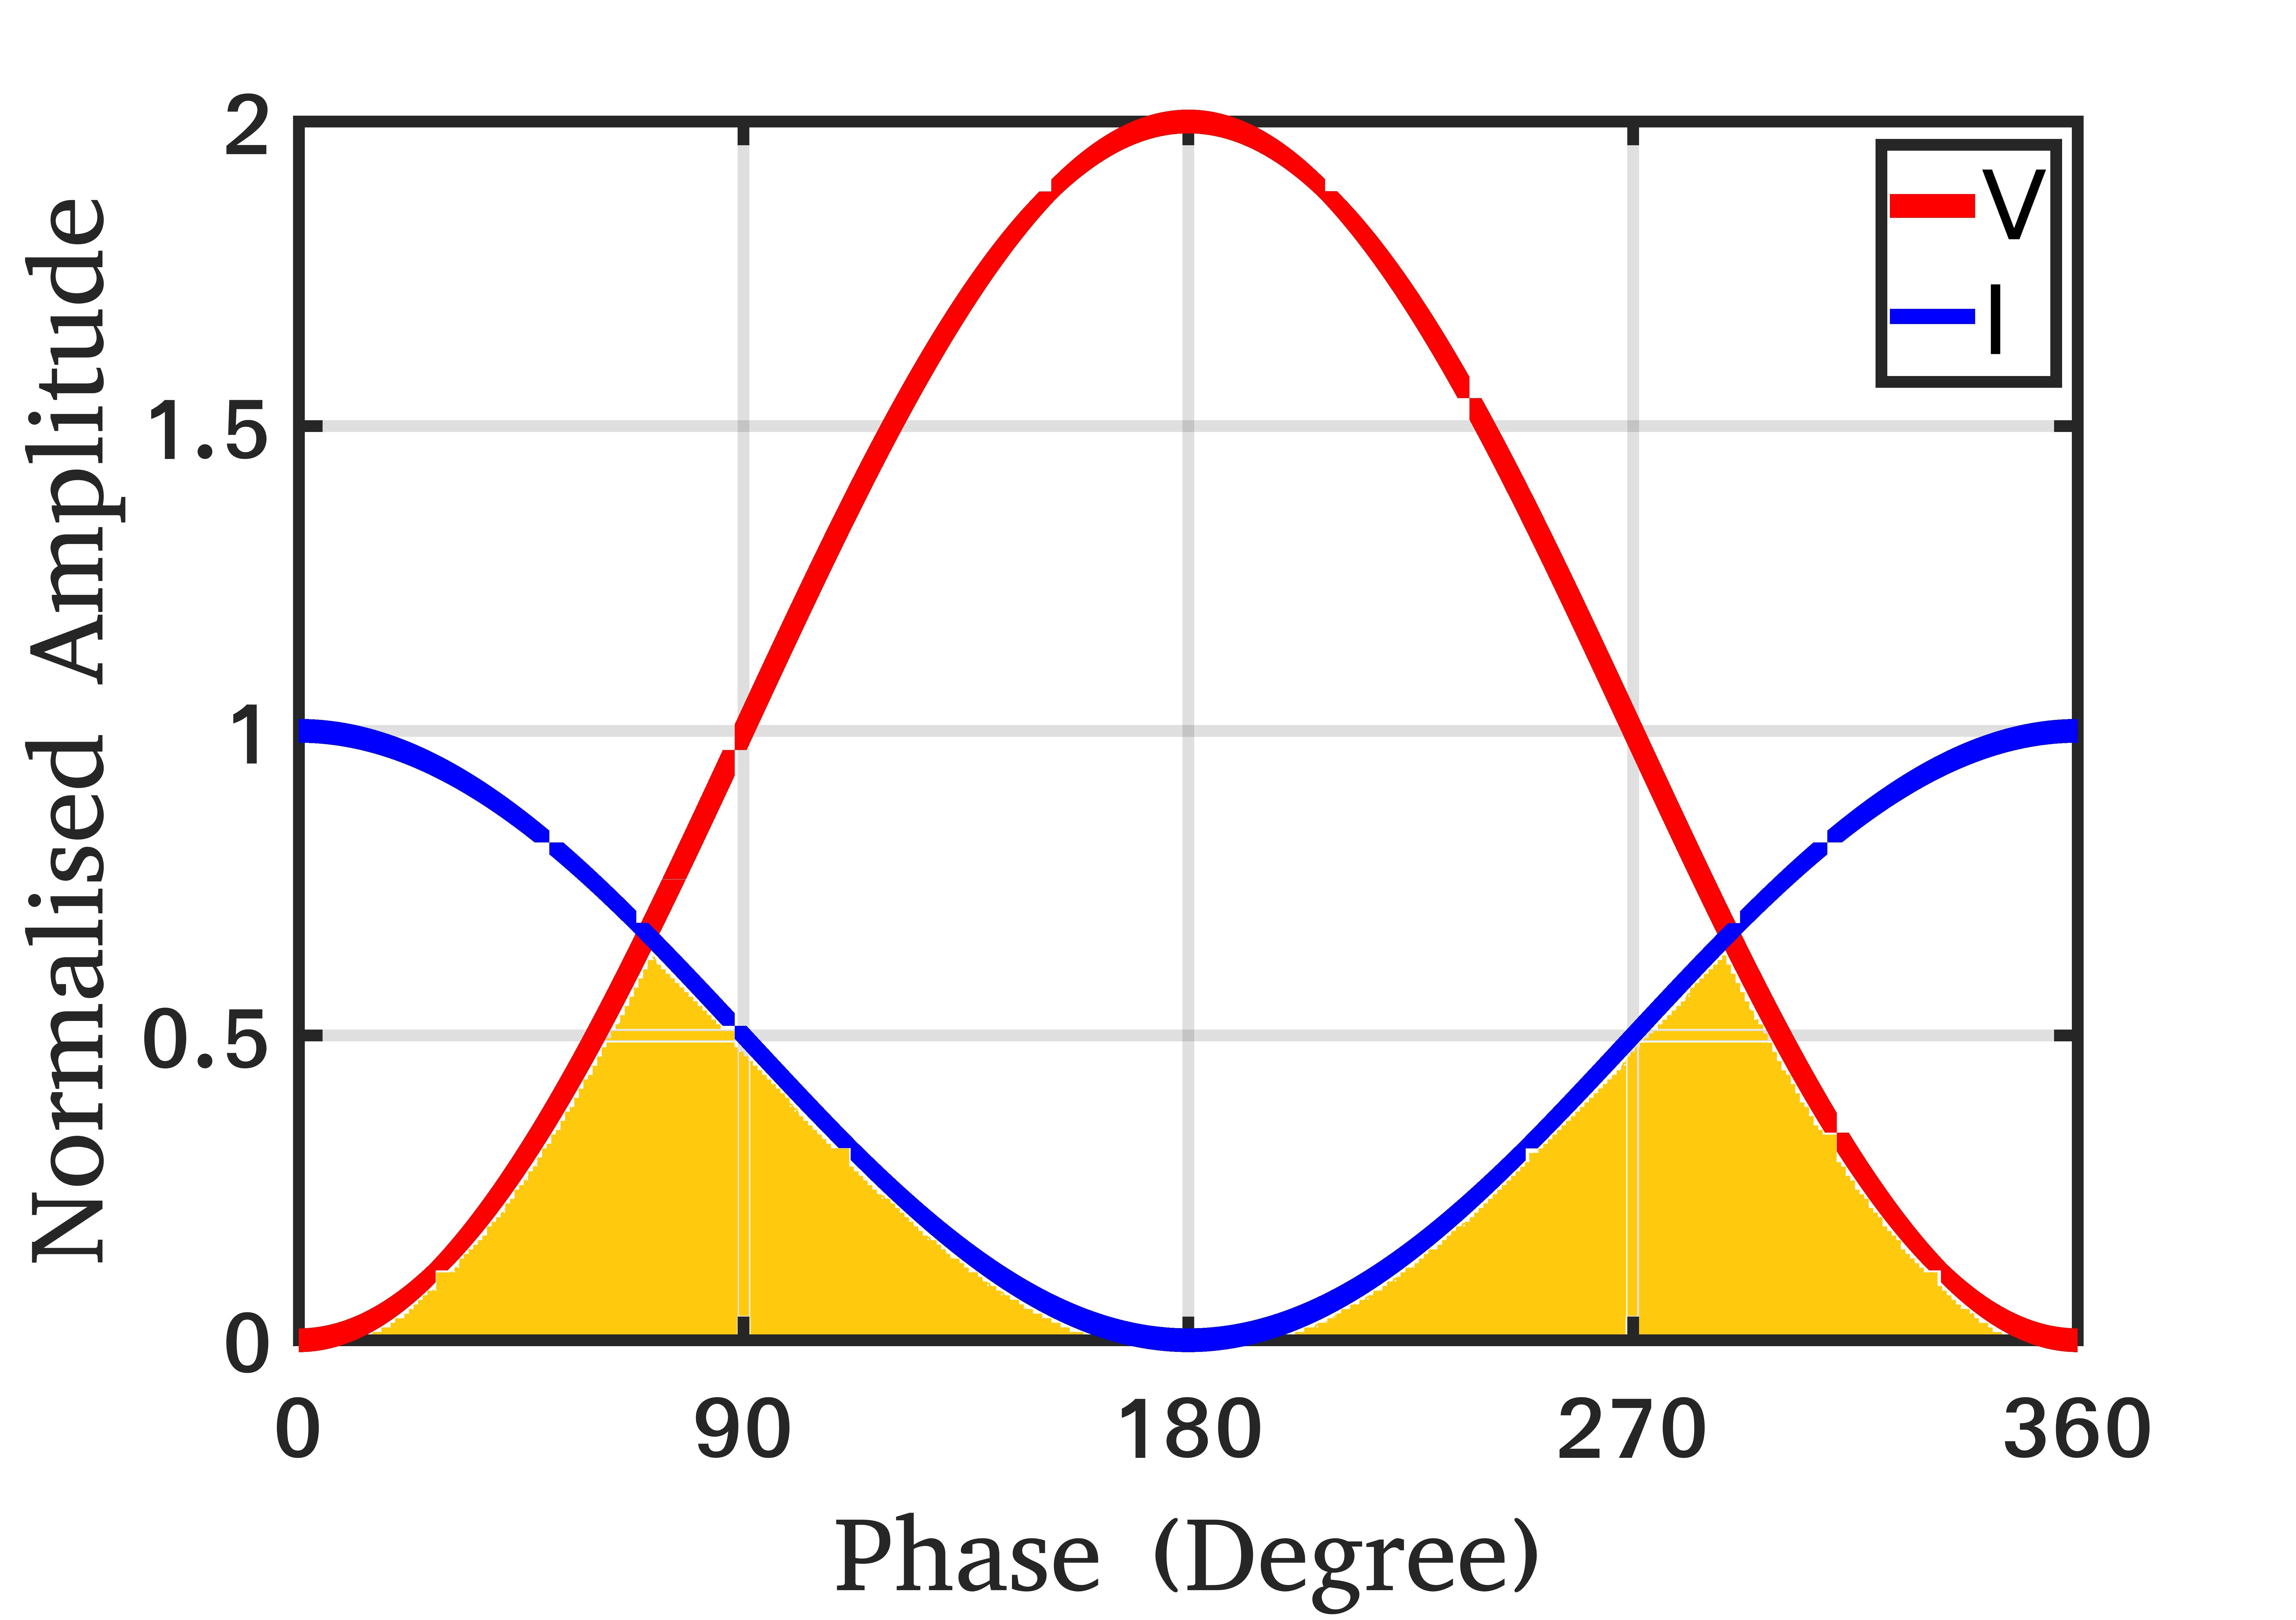
\includegraphics[width=0.9\textwidth]{Images/Intro/ClassA_shaded.jpg}
\caption{Class A}
\label{fig:CA_wave_VI}
\end{subfigure}
\begin{subfigure}{0.24\textwidth}
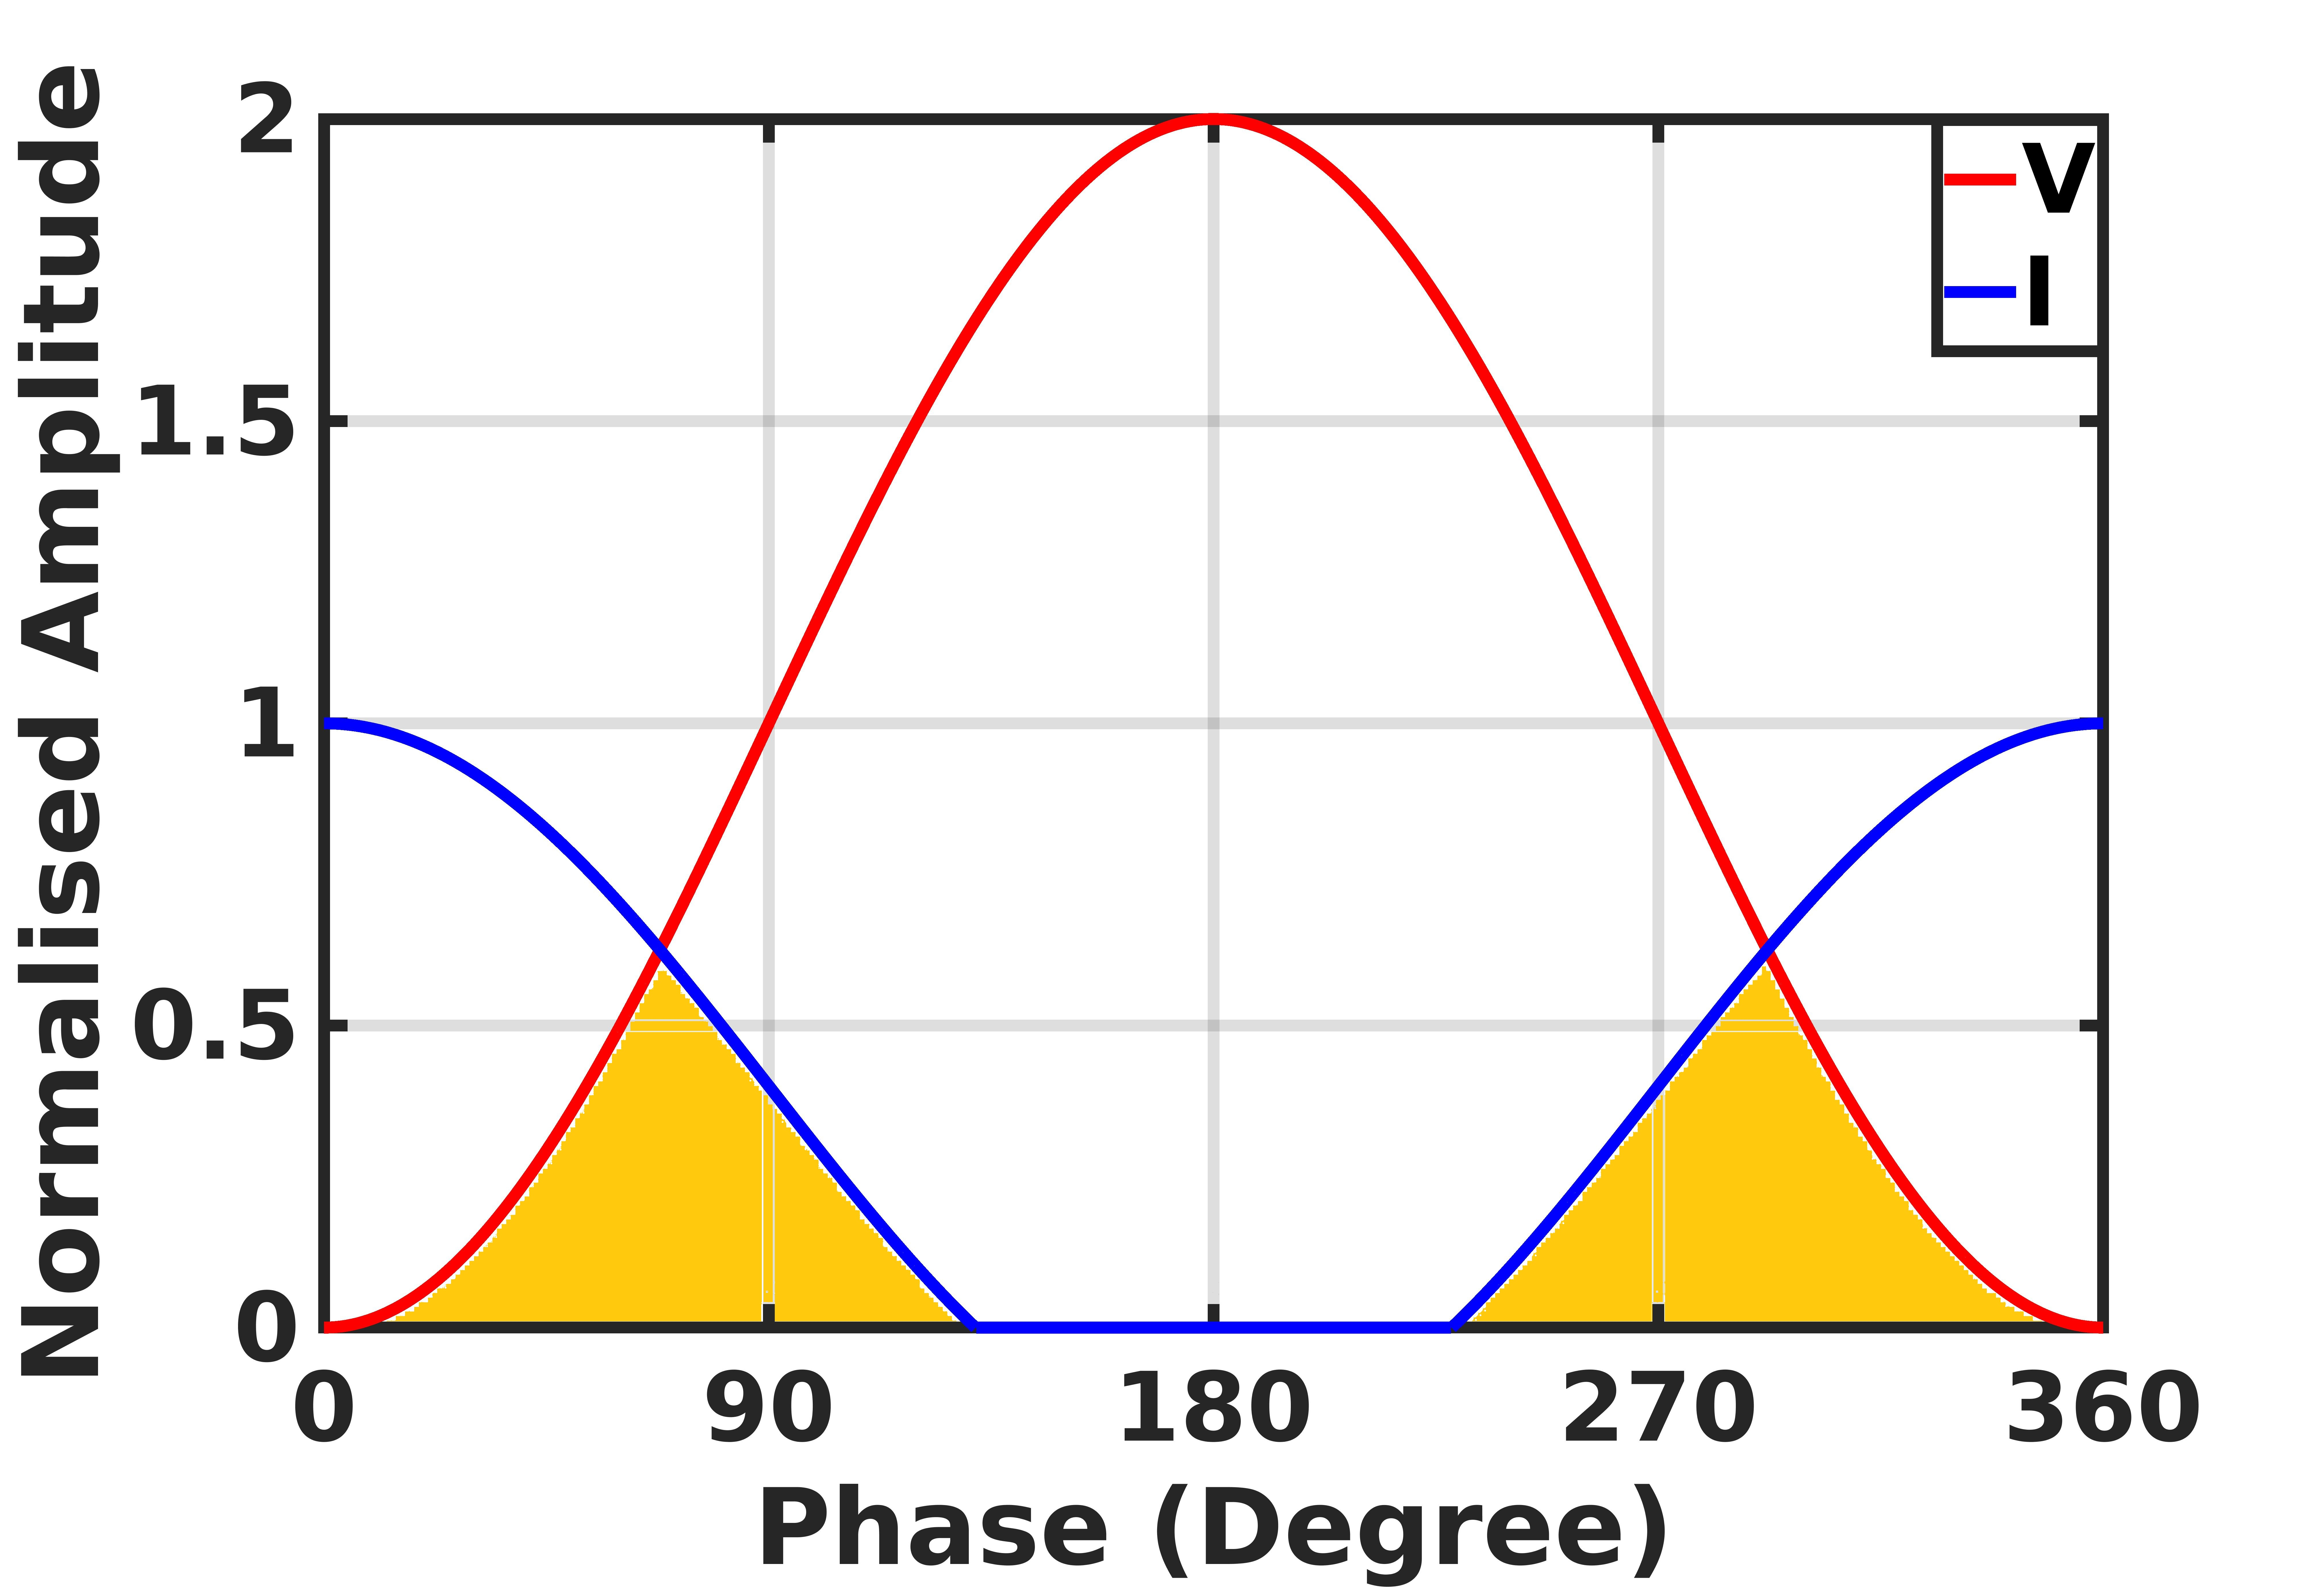
\includegraphics[width=0.9\textwidth]{Images/Intro/ClassB_shaded.jpg}
\caption{Class B}
\label{fig:CB_wave_VI}
\end{subfigure}
\begin{subfigure}{0.24\textwidth}
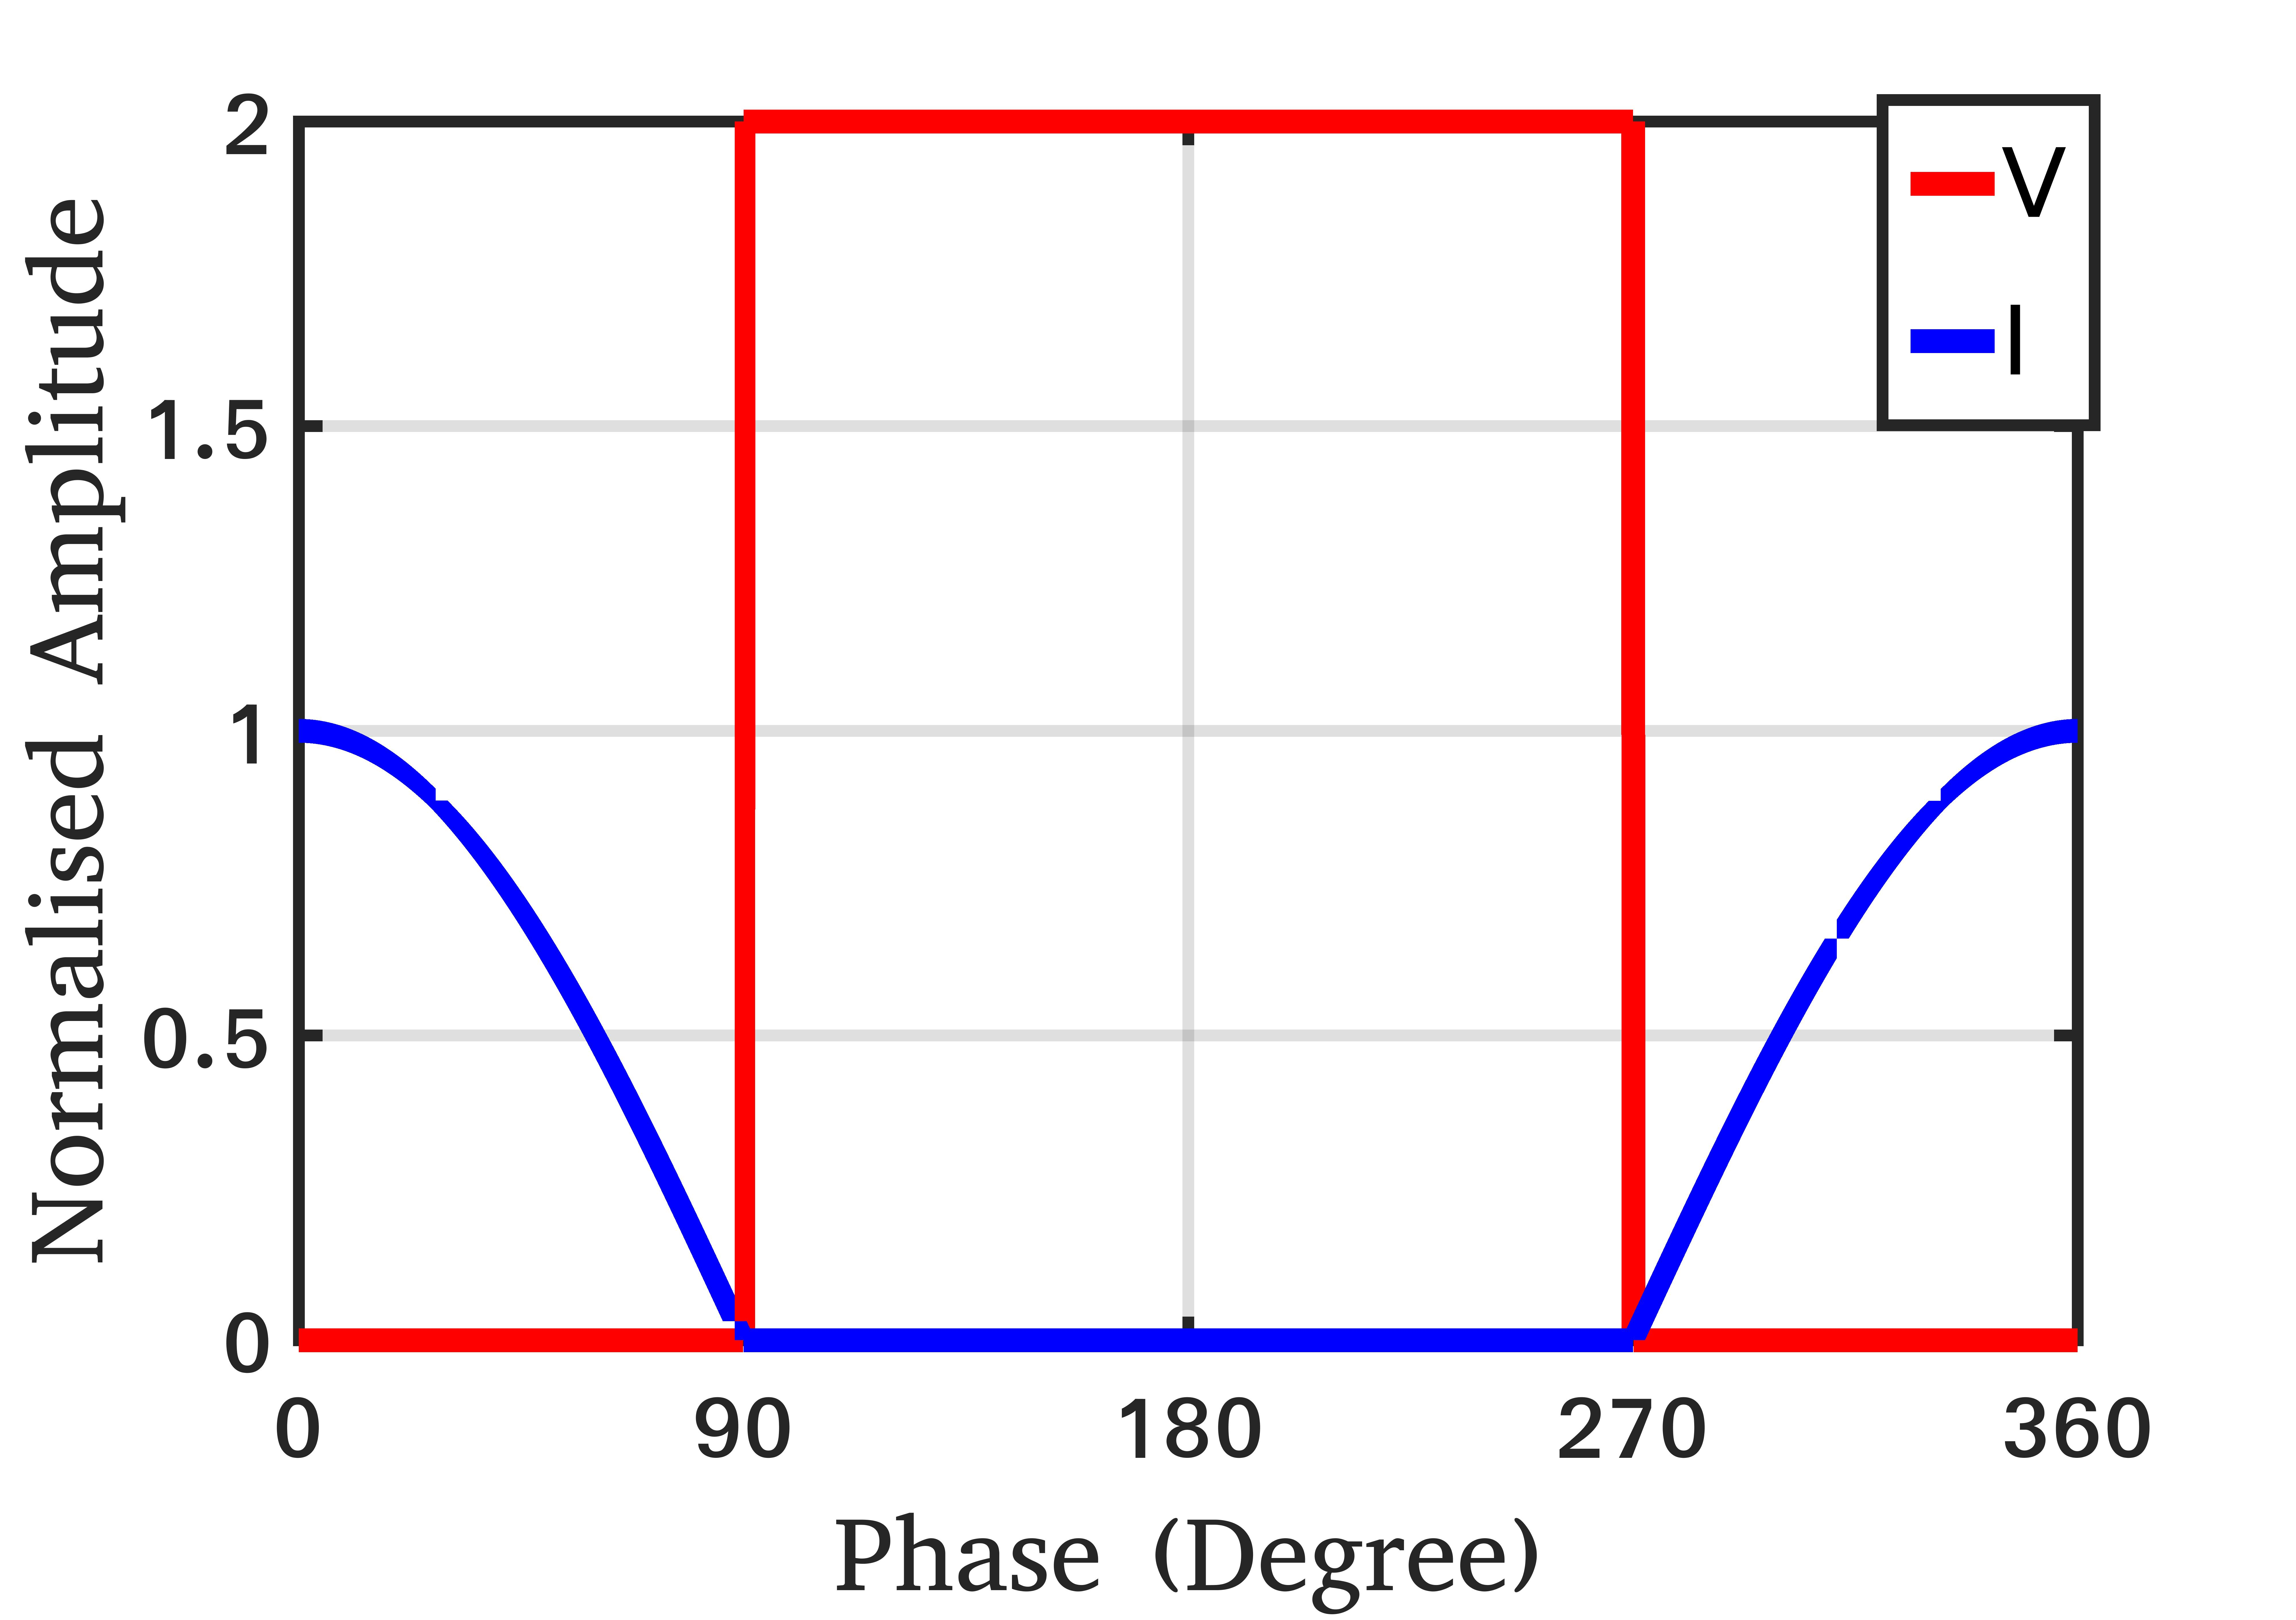
\includegraphics[width=0.9\textwidth]{Images/Intro/ClassF.jpg}
\caption{Ideal Class F}
\label{fig:ICF_wave_VI}
\end{subfigure}
\begin{subfigure}{0.24\textwidth}
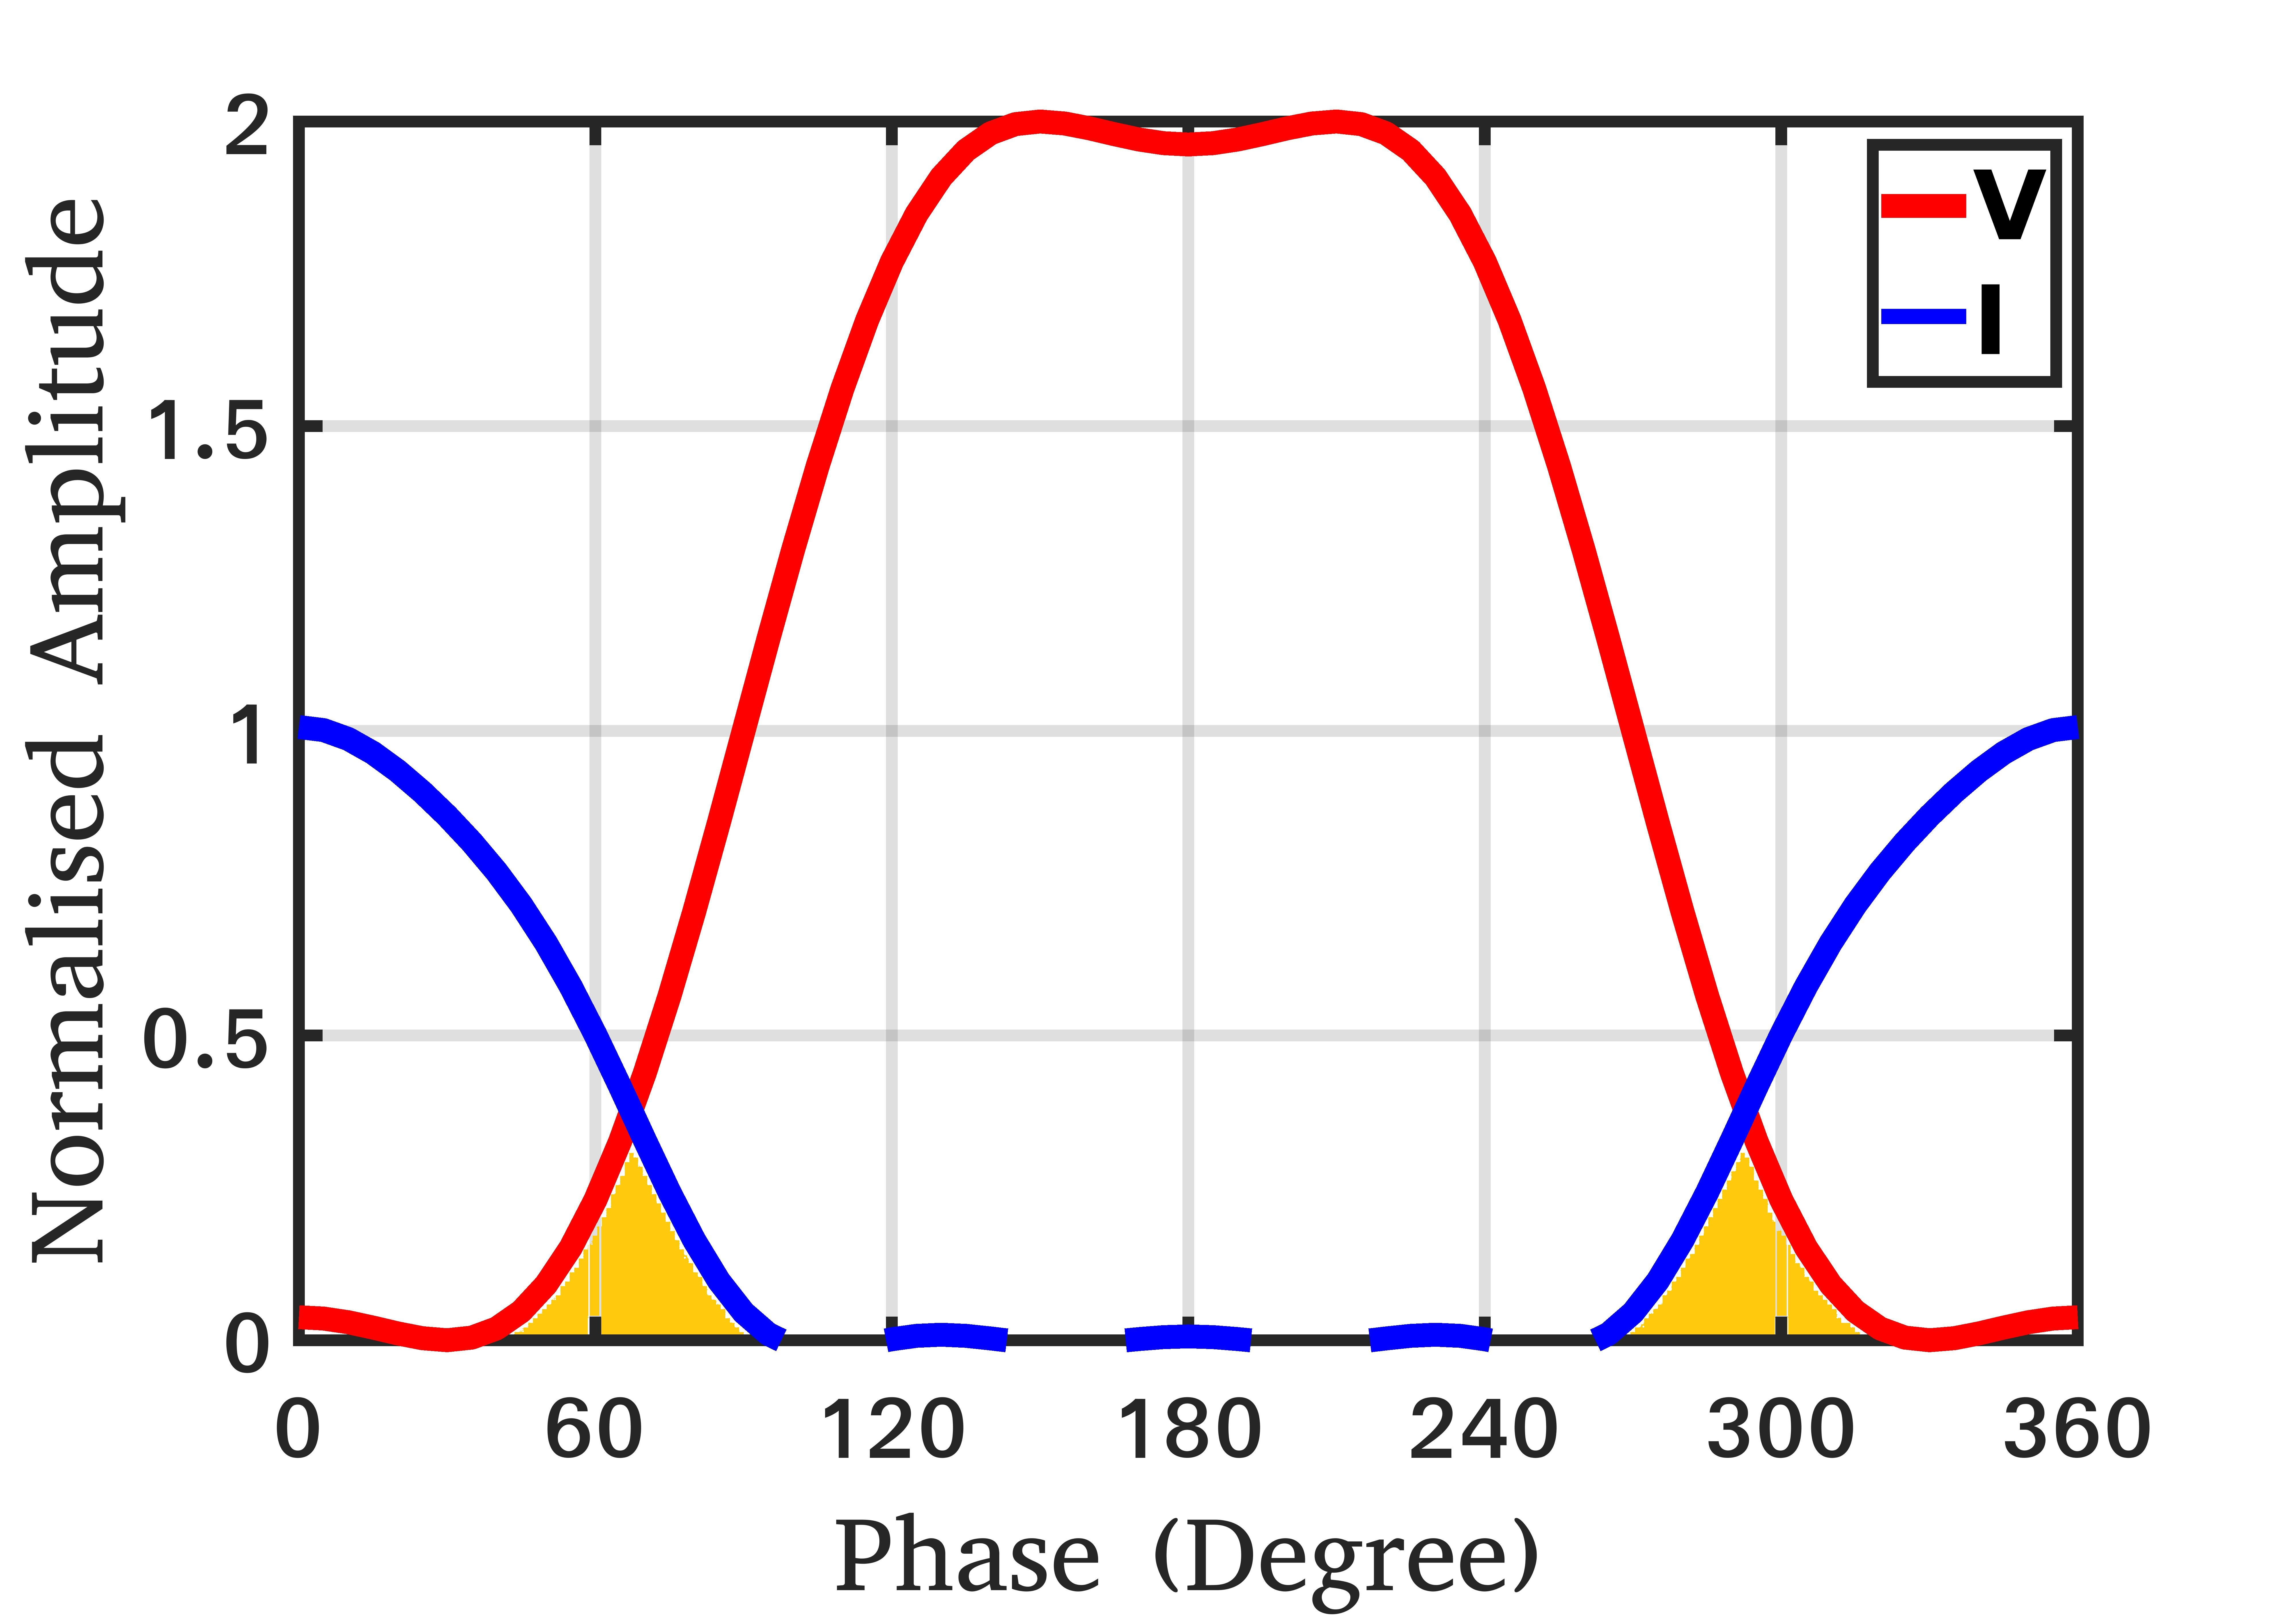
\includegraphics[width=0.9\textwidth]{Images/Intro/CF_wave_VI_shaded.jpg}
\caption{Practical Class F}
\label{fig:CF_wave_VI}
\end{subfigure}
\caption{Drain voltage (V) and drain current (I) waveform}
\label{fig:wave_VI}
\vspace{-0.25in}
\end{figure}
Generalized drain source voltage ($V_{DS}$) containing all frequencies up to $3^{rd}$ harmonic \cite{Gen_Vds_eqn} is given by:
\begin{equation}
V_{DS}=\underbrace{1}_{\text{DC}}-\underbrace{\frac{2}{\sqrt{3}} \cos \theta}_{\text{Fundamental}}+\underbrace{\frac{1}{3 \sqrt{3}} \cos 3 \theta}_{\text{$3^{rd}$ harmonic}}
\label{eqn_CF_V}
\end{equation}
Drain current ($I_{D}$) which is a half-sine wave is given by
\begin{equation}
I_{D}=\underbrace{\frac{1}{\pi}}_{\text{DC}}+\underbrace{\frac{1}{2} \cos \theta}_{\text{Fundamental}}+\underbrace{\frac{2}{3 \pi} \cos 2 \theta}_{\text{$2^{nd}$ harmonic}}-\underbrace{\frac{2}{15 \pi} \cos 4 \theta}_{\text{$4^{th}$ harmonic}}
\label{eqn_CCF_I}
\end{equation}
Load impedance in the fundamental, $2^{nd}$ and $3^{rd}$  harmonic bands are represented by $Z_{1f}$, $Z_{2f}$ and $Z_{3f}$ respectively.
\begin{equation}
\begin{aligned}
Z_{1f}=\frac{4}{\sqrt{3}}, \hspace{3mm}
Z_{2f}=0, \hspace{3mm}
Z_{3f}=\infty
\end{aligned}
\label{eqn_CF}
\end{equation}
Figure \ref{fig:CF_wave_VI} shows that the peak factor in class F is \textit{2}. Practical implementation of class F PA has a peak efficiency of \textit{90.7\%} but the main drawback is that they have limited bandwidths (typically \textit{10\%}) owing to the need for short and open circuit harmonic terminations. Thus, to realize wider bandwidth, the CCF PA has been proposed \cite{CCF_reason}.

The Section \ref{section:CCF} explains in brief the equation governing the operation of CCF. This is followed by Section \ref{section:ON} which discusses the procedure to design the different output networks for CCF. Then, the Section \ref{section:Results} comprises of the comparison results of \textit{4} proposed output network designs. Finally, Section \ref{section:Conclusion} concludes this paper.   

\section{Continuous Class F}
\label{section:CCF}
\vspace{-0.05in}
Compared to class F, the CCF has an imaginary part added at the fundamental and $2^{nd}$ harmonic of voltage waveform. So, the generalized $V_{DS}$ for CCF is given by \cite{ECCF_Carrubba}:
\begin{equation}
V_{DS}=\underbrace{1}_{\text{DC}}-\underbrace{\frac{2}{\sqrt{3}} \cos \theta-\gamma \sin \theta}_{\text{Fundamental}}+\underbrace{\frac{7 \gamma}{6 \sqrt{3}} \sin 2 \theta}_{\text{$2^{nd}$ harmonic}}+\underbrace{\frac{1}{3 \sqrt{3}} \cos 3 \theta}_{\text{$3^{rd}$ harmonic}}
\label{eqn_CCF_V}
\end{equation}
$I_{D}$ is a half sinusoid as in class F and given by Equation \ref{eqn_CCF_I}. It is seen that $V_{DS}$ and $I_{D}$ are chosen in such a way that no power is dissipated at higher harmonics. Also, the $\gamma$ in Equation \ref{eqn_CCF_V} doesn’t affect drain efficiency ($\eta_D$) mathematically. But the voltage waveform’s shape (peak factor) depends on $\gamma$ which is depicted in Figure \ref{fig:CCF_wave_VI}. 
But in reality, $I_{D}$ depends on $V_{DS}$, so $\eta_D$ reduces as $\gamma$ increases.

\begin{figure}[!t]
\centering
\captionsetup{font=footnotesize}
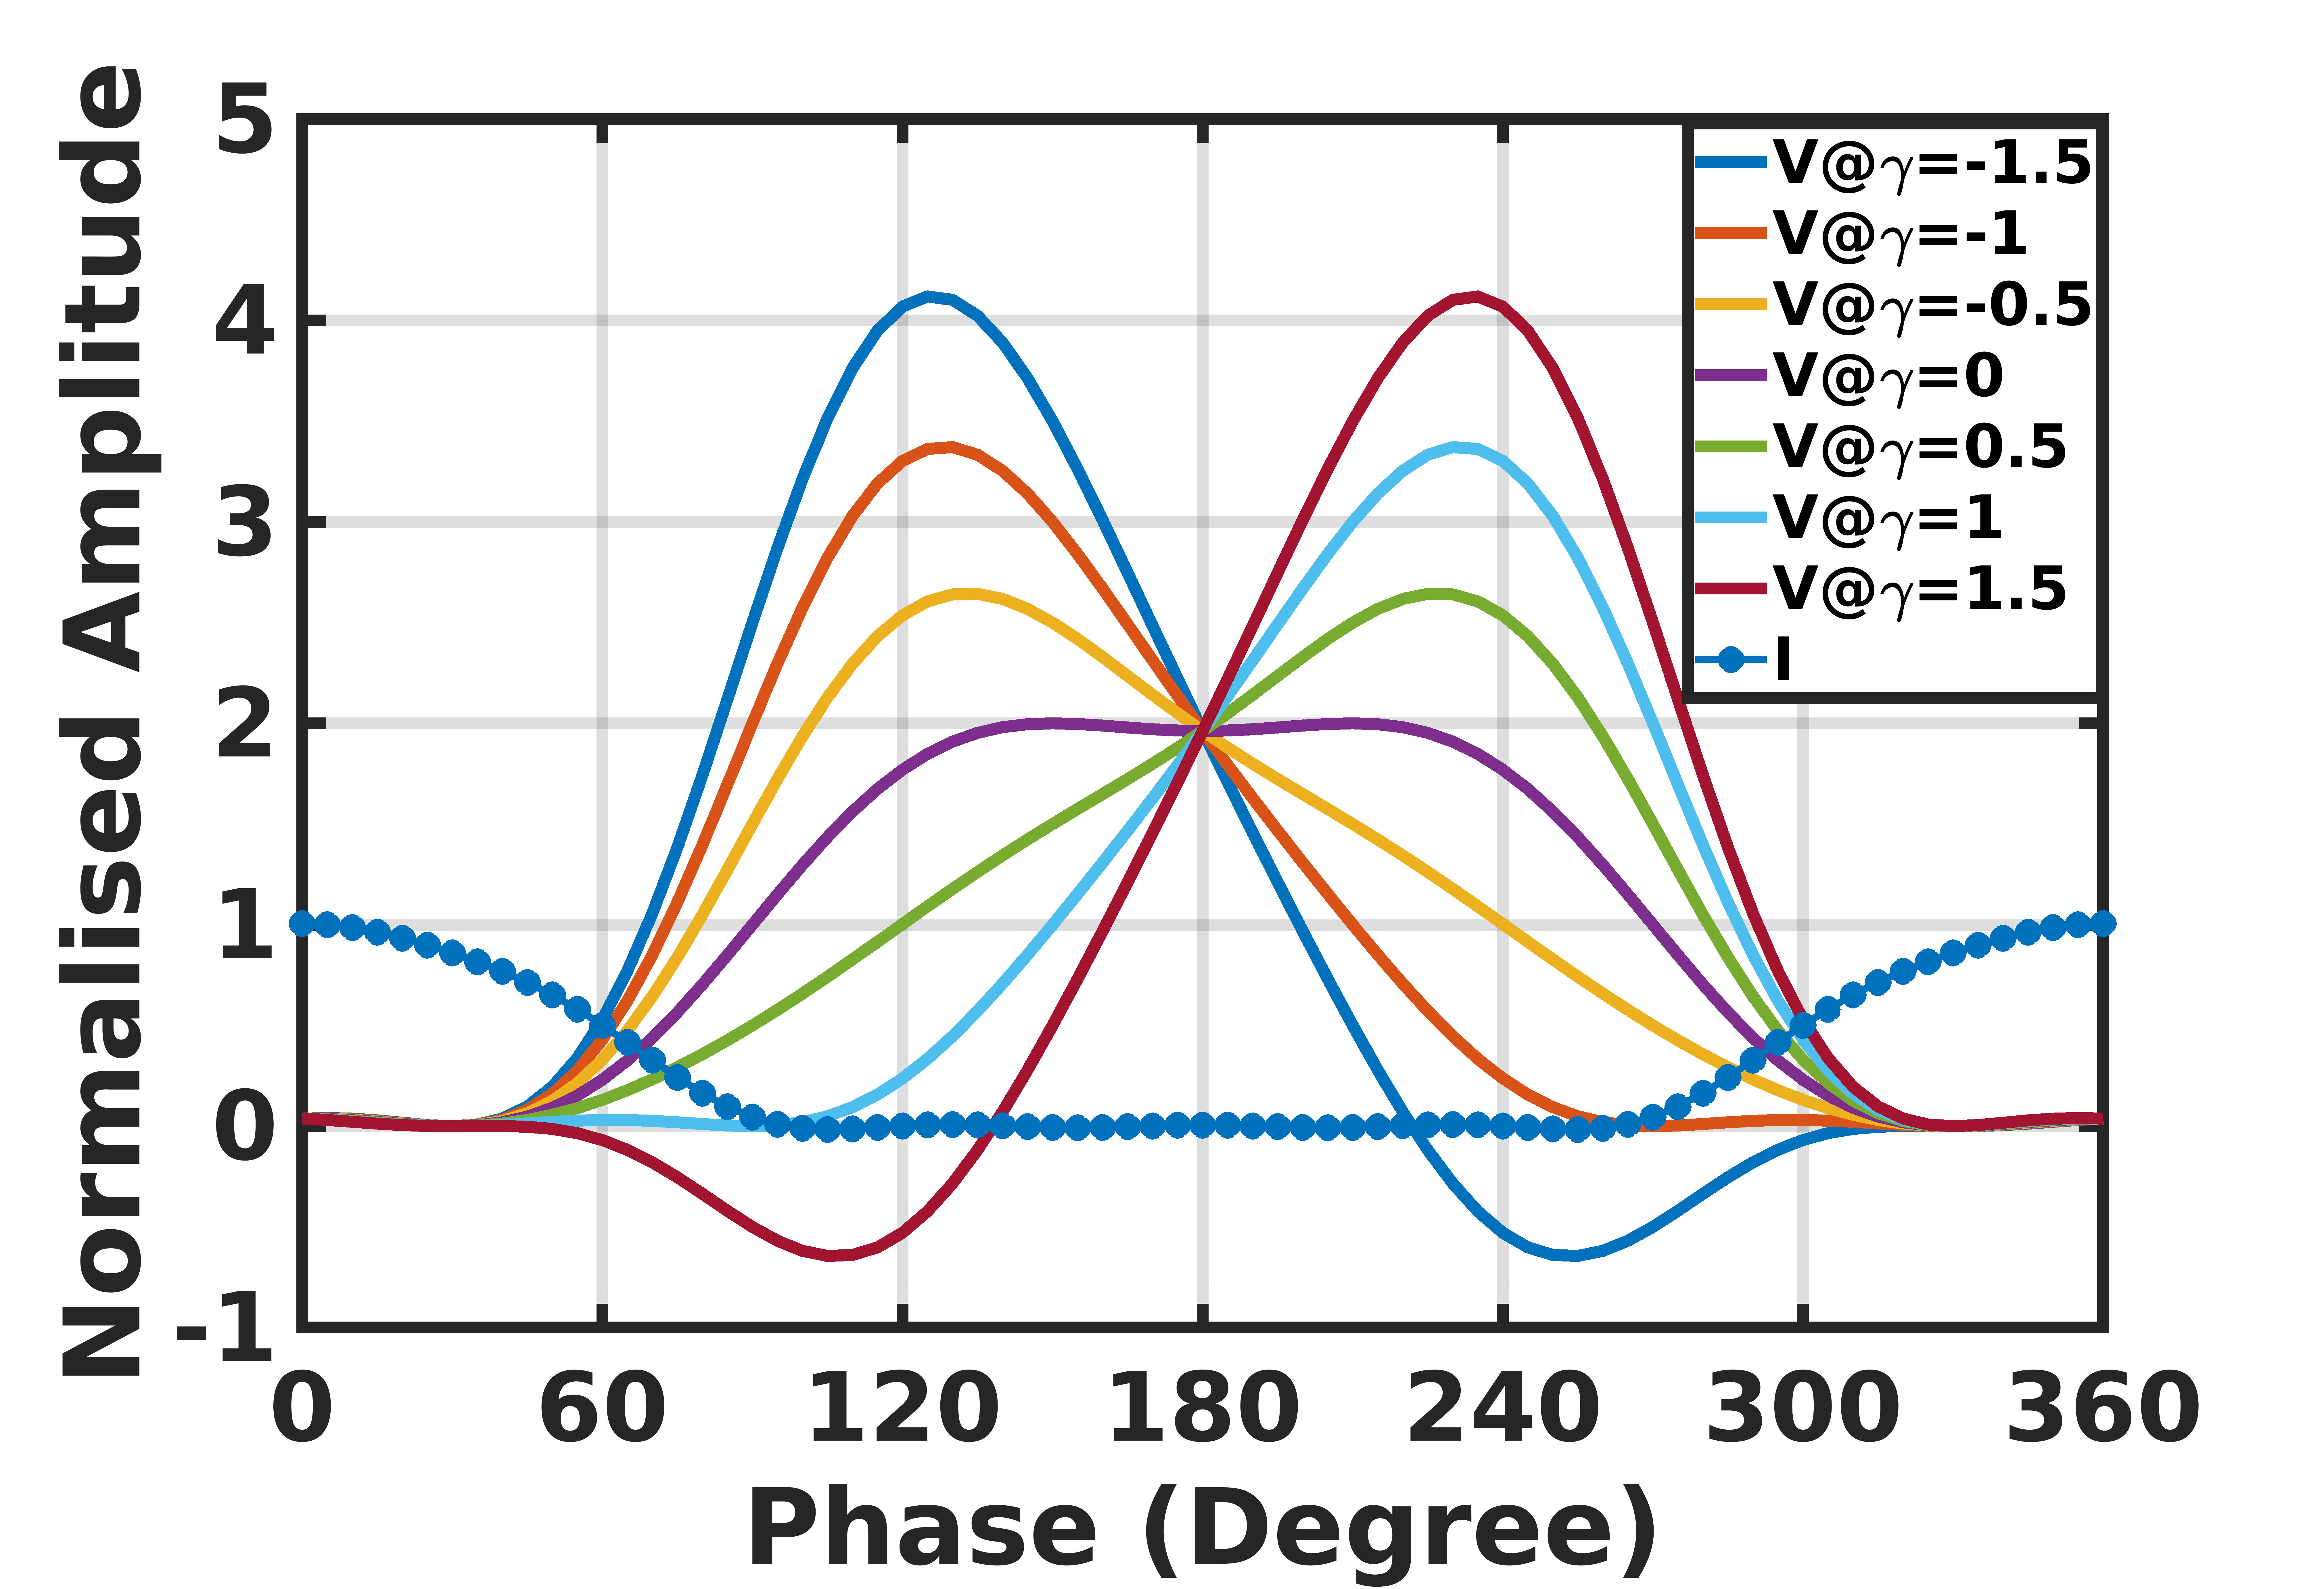
\includegraphics[width=3.4in, height=2in]{Images/CCF/CCF_wave_VI.jpg}
\caption{$V_{DS}$ and $I_D$ waveform for CCF with \textit{-1.5} $<$ $\gamma$ $<$ \textit{1.5}}
\label{fig:CCF_wave_VI}
\vspace{-0.25in}
\end{figure}

Figure \ref{fig:CCF_wave_VI} shows that at $\gamma$ = \textit{0}, waveform is like class F. For the $\gamma$ values between \textit{-1} and \textit{1}, $V_{DS}$ remains positive which enables CCF PA to have good linearity. One of the main downside of CCF PA is the increase in peak factor which reaches a value of \textit{3.12} times the supply ($V_{DD}$) when $\gamma$ = \textit{-1} or \textit{1}. 
Load impedance for CCF are calculated using Equations \ref{eqn_CCF_V} and \ref{eqn_CCF_I} \cite{CCFDesign_ali}.
\begin{equation}
\begin{aligned}
Z_{1f}=\frac{4}{\sqrt{3}}+j 2 \gamma, \hspace{2mm}
Z_{2f}=0-j \frac{\pi}{2} \frac{7 \sqrt{3}}{6} \gamma,\hspace{2mm}
Z_{3f}=\infty
\label{eqn_CCF_imp}
\end{aligned}
\end{equation}

In CCF, $Z_{3f}$ remains open-circuited similar to class F. Meanwhile, $Z_{1f}$ and $Z_{2f}$ has a reactive part, unlike Class F. From the Equation \ref{eqn_CCF_imp} and Figure \ref{fig:CCF_SC}, it is observed that if the reactive part of $Z_{1f}$ changes from inductive to capacitive, then the reactive part of $Z_{2f}$ need to change from capacitive to inductive or vice-versa across the bandwidth to achieve CCF operation. In the next section, the design procedure for the \textit{4} output networks is illustrated step by step.

\begin{figure}[!t]
\centering
\captionsetup{font=footnotesize}
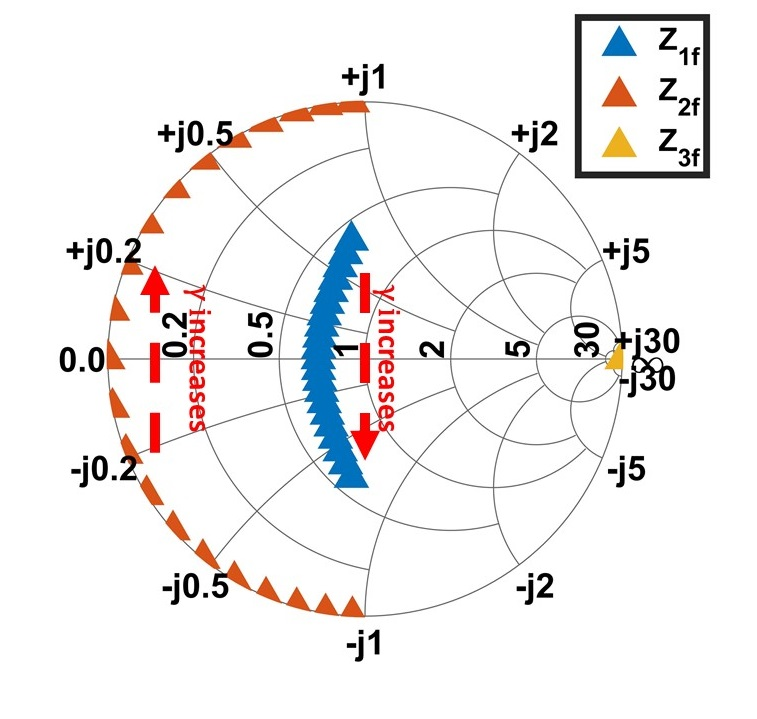
\includegraphics[width=0.8\linewidth]{Images/CCF/CCF_SC.jpg}
\caption{Variation of $Z_{1f}$, $Z_{2f}$, $Z_{3f}$ for \textit{-1} $<$ $\gamma$ $<$ \textit{1}}
\label{fig:CCF_SC}
\vspace{-0.05in}
\end{figure}
 

\section{Design of Output Network for CCF}
\label{section:ON}
In this paper, the differential structure is chosen for the PA mainly because it helps to decouple the design of $2^{nd}$ harmonic impedance with the fundamental and $3^{rd}$ harmonic impedance. Moreover, it also helps to reduce common-mode noise, substrate coupling, and second-order nonlinearities as well as double the output power compared to single-ended. 
The PA in this paper is designed for a peak power of \textit{27 dBm} for the operational bandwidth of \textit{2.1 - 2.7 GHz} with $V_{DD}$ = \textit{2.7 V} and to achieve this, a differential impedance of \textit{38.7} $\Omega$ should be presented to the drains of the transistors at fundamental across the entire bandwidth (refer Equation \ref{eqn_diff_imp}). 
\vspace{-0.1in}
\begin{equation}
\begin{aligned}
&V_{FUND}(de)=2*V_{FUND}(se)=2*\frac{2}{\sqrt{3}} V_{DD}=6.24 \hspace{1mm}V\\
&R_{D}(de)=\frac{V_{FUND}(de)^{2}}{2*\text{Peak} \hspace{1mm} P_{OUT}}=38.7 \hspace{1mm} \Omega
\label{eqn_diff_imp}
\end{aligned}
\end{equation}
The requirements of the output network for CCF is exhibited in Table \ref{tab:Output_Network_Requirements}. The PA operates in Class F mode at the center frequency $\omega_0$ (\textit{2.4 GHz}) with a short at $2\omega_0$ (\textit{4.8 GHz}) and an open at $3\omega_0$ (\textit{7.2 GHz}). But, for all other frequencies, the PA performs in the CCF mode. 

\setlength{\arrayrulewidth}{0.5mm}
\setlength{\tabcolsep}{2pt}
\renewcommand{\arraystretch}{1.5}
\begin{table}[!t]
\centering
\captionsetup{font=footnotesize}
\resizebox{\linewidth}{!}{%
\begin{tabular}{|c|c|c|c|}
\hline
\textbf{Class of Operation} & \begin{tabular}[c]{@{}c@{}}\textbf{First Harmonic} ($\omega$)\end{tabular} & \begin{tabular}[c]{@{}c@{}}\textbf{Second Harmonic} (2$\omega$)\end{tabular} & \begin{tabular}[c]{@{}c@{}}\textbf{Third Harmonic} (3$\omega$)\end{tabular} \\ \hline
\multirow{2}{*}{\textbf{\begin{tabular}[c]{@{}c@{}}Class F \\ (2.4 GHz)\end{tabular}}} & $\Re(Z_D)$ = 38.7 $\Omega$ & $\Re(Z_D)$= 0 $\Omega$ & \multirow{2}{*}{\begin{tabular}[c]{@{}c@{}}$|Z_D|$ needs to be high \end{tabular}} \\ \cline{2-3}
 & $\Im(Z_D)$ = 0 $\Omega$ & $\Im(Z_D)$ = 0 $\Omega$ &  \\ \hline
\multirow{2}{*}{\textbf{\begin{tabular}[c]{@{}c@{}}\\CCF \\ (2.1 - 2.7 GHz)\end{tabular}}} & $\Re(Z_D)$ = 38.7 $\Omega$ & $\Re(Z_D)$ = 0 $\Omega$ & \multirow{2}{*}{\begin{tabular}[c]{@{}c@{}}\\$|Z_D|$ needs to be high \end{tabular}} \\ \cline{2-3}
 & \begin{tabular}[c]{@{}c@{}}$\Im(Z_D)$ need to change from + to -\\ OR\\ $\Im(Z_D)$ need to change from - to +\end{tabular} & \begin{tabular}[c]{@{}c@{}} $\Im(Z_D)$ need to change from - to +\\ OR\\ $\Im(Z_D)$ need to change from + to -\end{tabular} &  \\ \hline
\end{tabular}%
 }
\caption{Output network specifications}
\label{tab:Output_Network_Requirements}
\vspace{-0.25in}
\end{table}

Figures \ref{fig:Design_A_FC}, \ref{fig:Design_B_FC}, \ref{fig:Design_C_FC}, and \ref{fig:Design_D_FC} shows the schematics of \textit{4} output networks which are designed using lossless lumped components.. 
All the designs have a balun and a load capacitance ($C_L$), because the balun converts differential-ended signal to single-ended signal as the load is single-ended, whereas $C_L$ shorts the $R_L$ (\textit{50} $\Omega$) at $3^{rd}$ harmonic to obtain high impedance. Drain source capacitance of the transistor (Assumed $C_{DS}=1.87\hspace{1mm}pF$) is absorbed into the output network to reduce its impact on the PA performance. The balun is modelled using ideal transformer, magnetizing inductance ($L_m$), leakage inductance ($L_k$), primary inductance ($L_P$) and coupling coefficient ($km$) \cite{Transformer_model}. 

\subsection{Design A (no RF choke \& with $L_2C_2$)}
Design A consists of a second harmonic trap ($L_2C_2$) which provides short at $2\omega_0$. The $V_{DD}$ is provided through the center tap of the balun and $L_{BND}$ is used to model bond-wire inductance ($\approx$ \textit{1 nH}).
Analysis of the schematics is done in differential and common mode by using the equivalent circuit shown in Figure \ref{fig:Design_A_Diff} and \ref{fig:Design_A_Com} respectively to calculate the unknown parameters: $km$, transformer's turn ratio ($N$), $L_P$, $C_2$, $L_2$, and $C_L$.
\begin{figure}[!t]
\captionsetup{font=footnotesize}
\centering
\begin{subfigure}{0.5\textwidth}
\centering
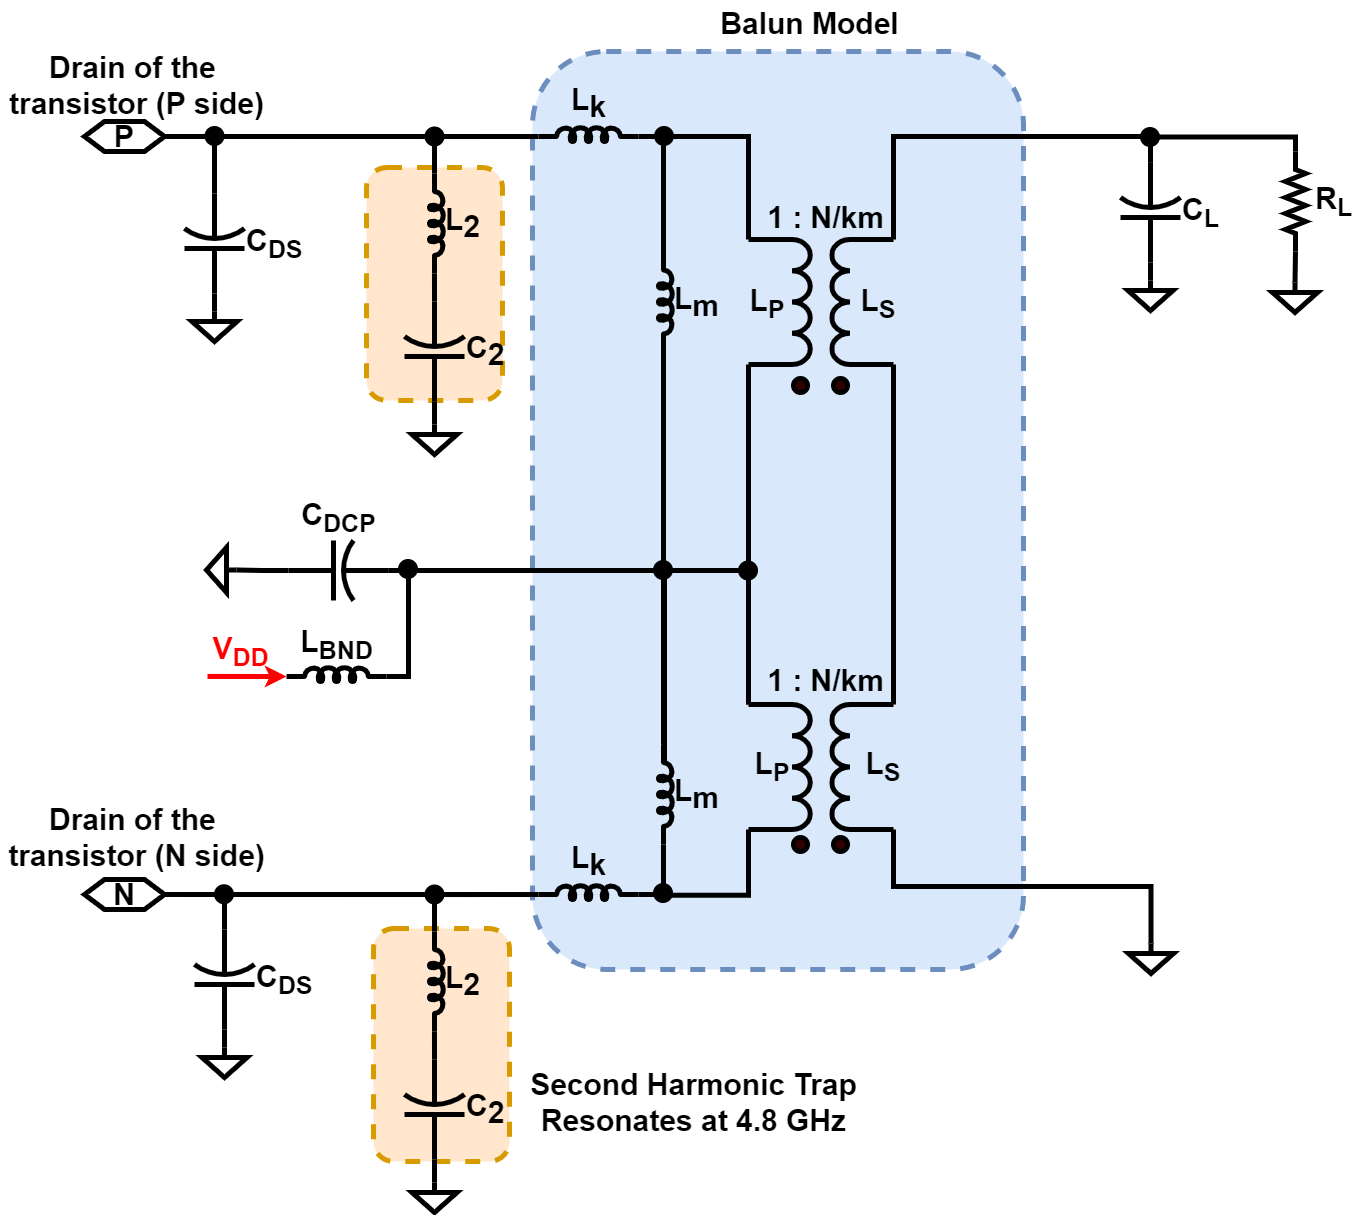
\includegraphics[width=0.5\textwidth]{Images/Design/Design_A_FC.png}
\caption{Schematics}
\label{fig:Design_A_FC}
\end{subfigure}
\begin{subfigure}[b]{0.24\textwidth}
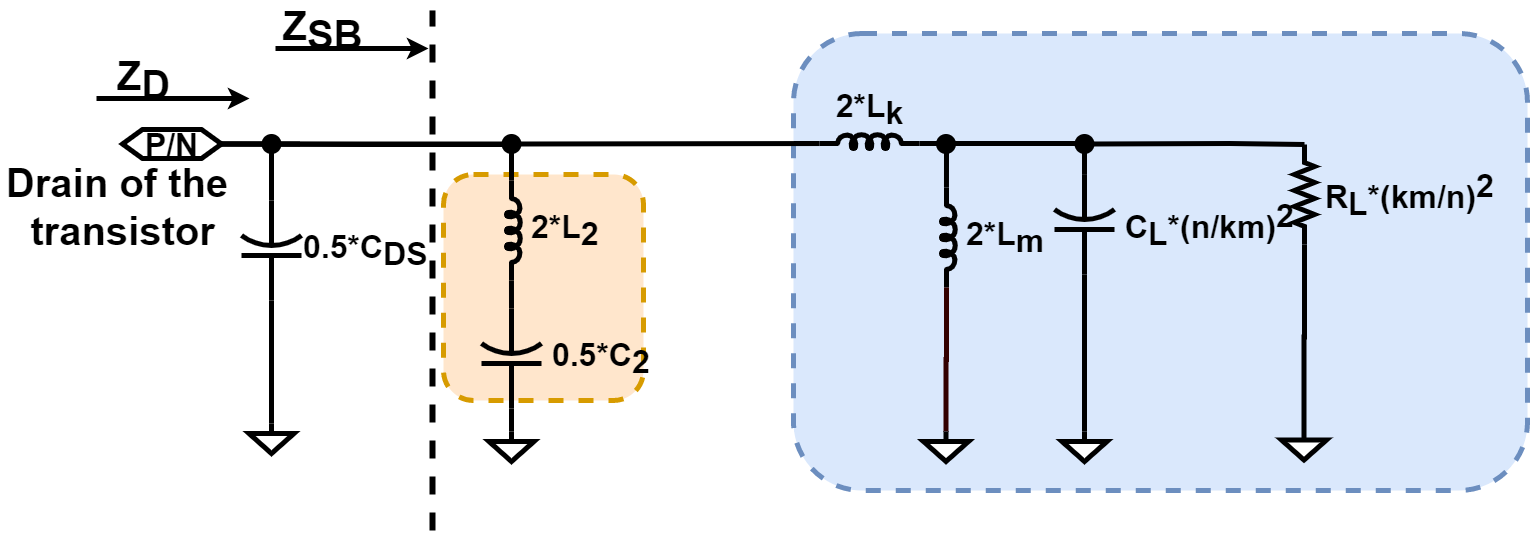
\includegraphics[width=1\textwidth]{Images/Design/Design_A_Diff.png}
\caption{Differential mode equivalent circuit}
\label{fig:Design_A_Diff}
\end{subfigure}
\begin{subfigure}[b]{0.24\textwidth}
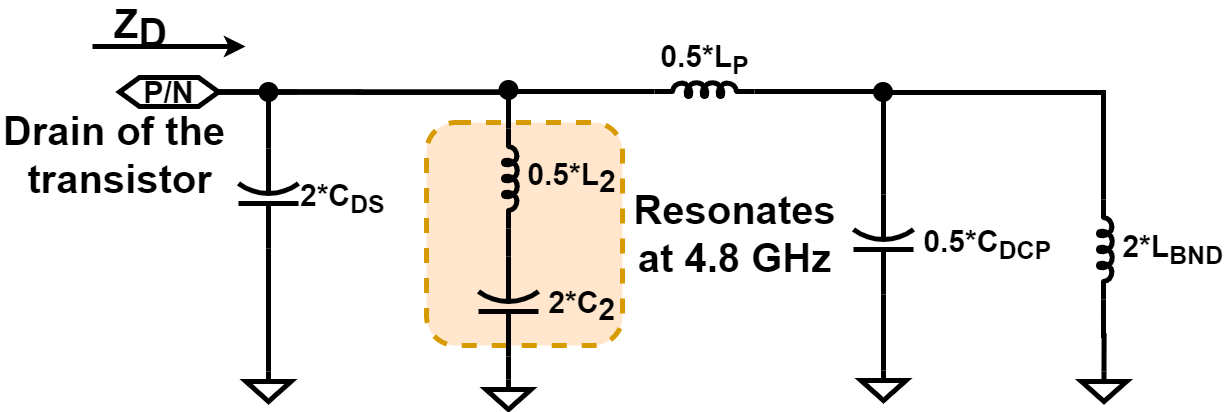
\includegraphics[width=1\textwidth]{Images/Design/Design_A_Com.png}
\caption{Common mode equivalent circuit}
\label{fig:Design_A_Com}
\end{subfigure}
\caption{Design A (Balun, $L_2C_2$ and $C_L$)}
\label{fig:Design_A}
\vspace{-0.3in}
\end{figure}
Figure \ref{fig:Design_A_Diff} shows that the drain impedance ($Z_D$) is given by
\begin{equation}
    Z_D=(\frac{1}{\frac{j\omega C_{DS}}{2}}+\frac{1}{Z_{SB}})^{-1}=38.7 \hspace{1mm} \Omega
    \label{eqn:ZD}
\end{equation}
The value of $Z_{SB}$ (impedance of $L_2C_2$ and balun given by equation \ref{eqn:Design_A_ZSB}) that will provide $Z_D$ of \textit{38.7} $\Omega$ can be calculated from equation \ref{eqn:ZD} and the value is $\Re(Z_{SB})(\omega_0) =  29.8\hspace{1mm} \Omega$ and $\Im(Z_{SB})(\omega_0) = 16.6\hspace{1mm}\Omega$.

\begin{equation}
\begin{aligned}
    &Z_{SB}=(\frac{1}{Z_B}+\frac{1}{Z_S})^{-1}
    \hspace{1mm}\text{where}, Z_S=2j\omega  L_2+\frac{1}{\frac{j \omega C_2}{2}}, \\
    &Z_B=(\frac{1}{R_P}+\frac{1}{2j \omega  L_m}+j \omega C_P)^{-1}+2j \omega  L_k,\\ &R_P=R_L(\frac{km}{n})^2,C_P=C_L(\frac{n}{km})^2
\label{eqn:Design_A_ZSB}
\end{aligned}
\end{equation}

From equation \ref{eqn:ZD}, it is evident that $C_{DS}$ should resonate out with $\Im(Z_{SB})$  to attain high drain impedance at $3\omega_0$. This implies $\Im(Z_{SB})(3\omega_0) = 24.96\hspace{1mm}\Omega$.
Ideally, $\Re(Z_{SB})(3\omega_0)$ should be \textit{0} to achieve high $3^{rd}$ harmonic impedance, but Figure \ref{fig:Design_A_Rn_var_1H} depicts that having a larger $\Re(Z_{SB)}(3\omega_0)$ helps to get a constant $P_{OUT}$ across the operational bandwidth by having a flatter real part at the fundamental. Another benefit is that it has more linear reactive part at the fundamental which helps in CCF operation.
However, this leads to a lower $3^{rd}$ harmonic impedance as showcased in Figure \ref{fig:Design_A_Zn_3H}. This also emphasizes  the significance of $C_L$. So, to achieve \textit{1000} $\Omega$ at $3^{rd}$ harmonic,  $\Re(Z_{SB})(3\omega_0) = 0.5\hspace{1mm}\Omega$ which is obtained from Figure \ref{fig:Design_A_Zn_3H}. Figure \ref{fig:Design_A_Com} proves that $L_2$ should  should have a series resonance with $C_2$ to get short at 2$\omega_0$.

\begin{equation}
    L_2=\frac{1}{4*\omega_0^2*C_2}%=0.73 \hspace{1mm} nH
    \label{eqn:Design_A_2H}
\end{equation}

\begin{figure}[!t]
\captionsetup{font=footnotesize}
\centering
\begin{subfigure}{0.24\textwidth}
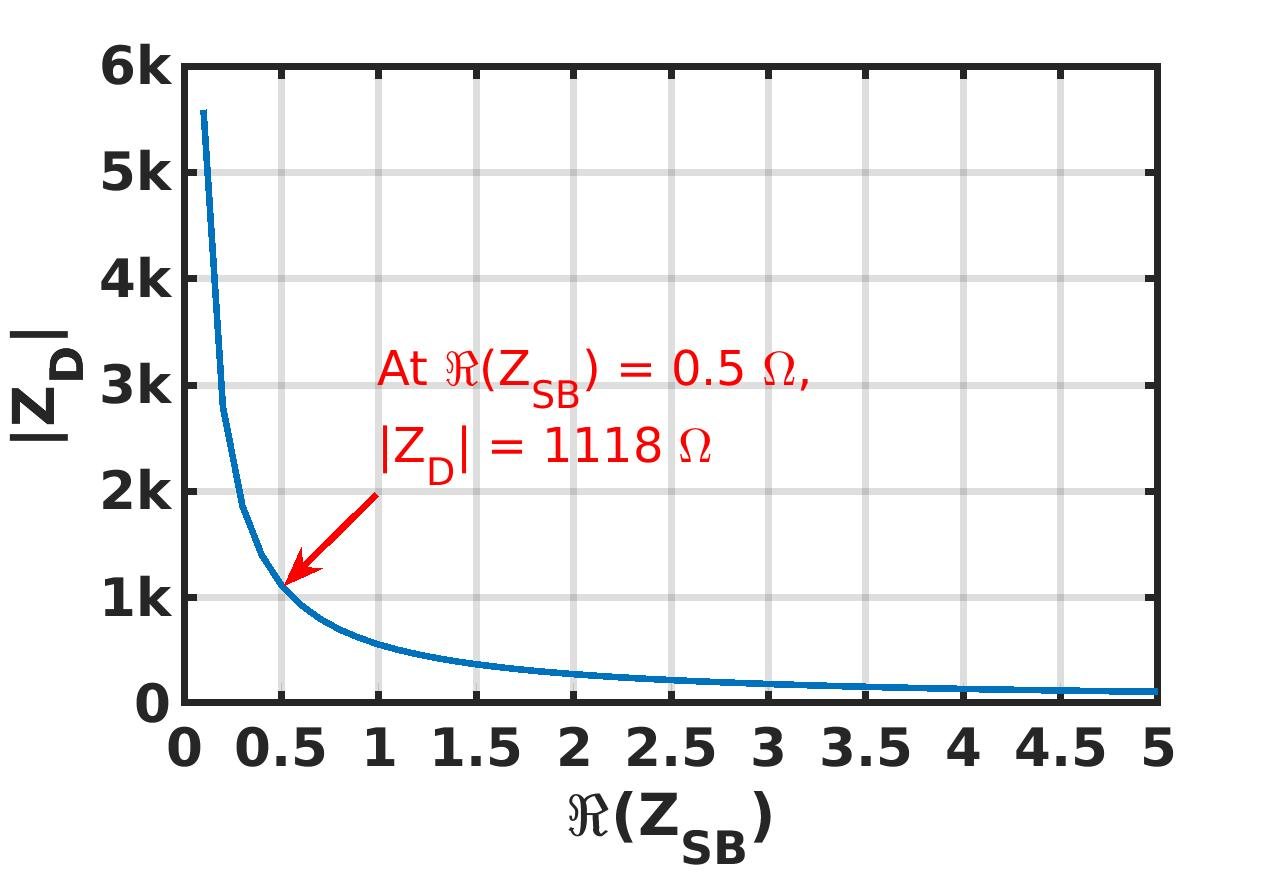
\includegraphics[width=1\textwidth]{Images/Design/Design_A_Zn_3H.jpg}
\caption{}
\label{fig:Design_A_Zn_3H}
\end{subfigure}
\begin{subfigure}{0.24\textwidth}
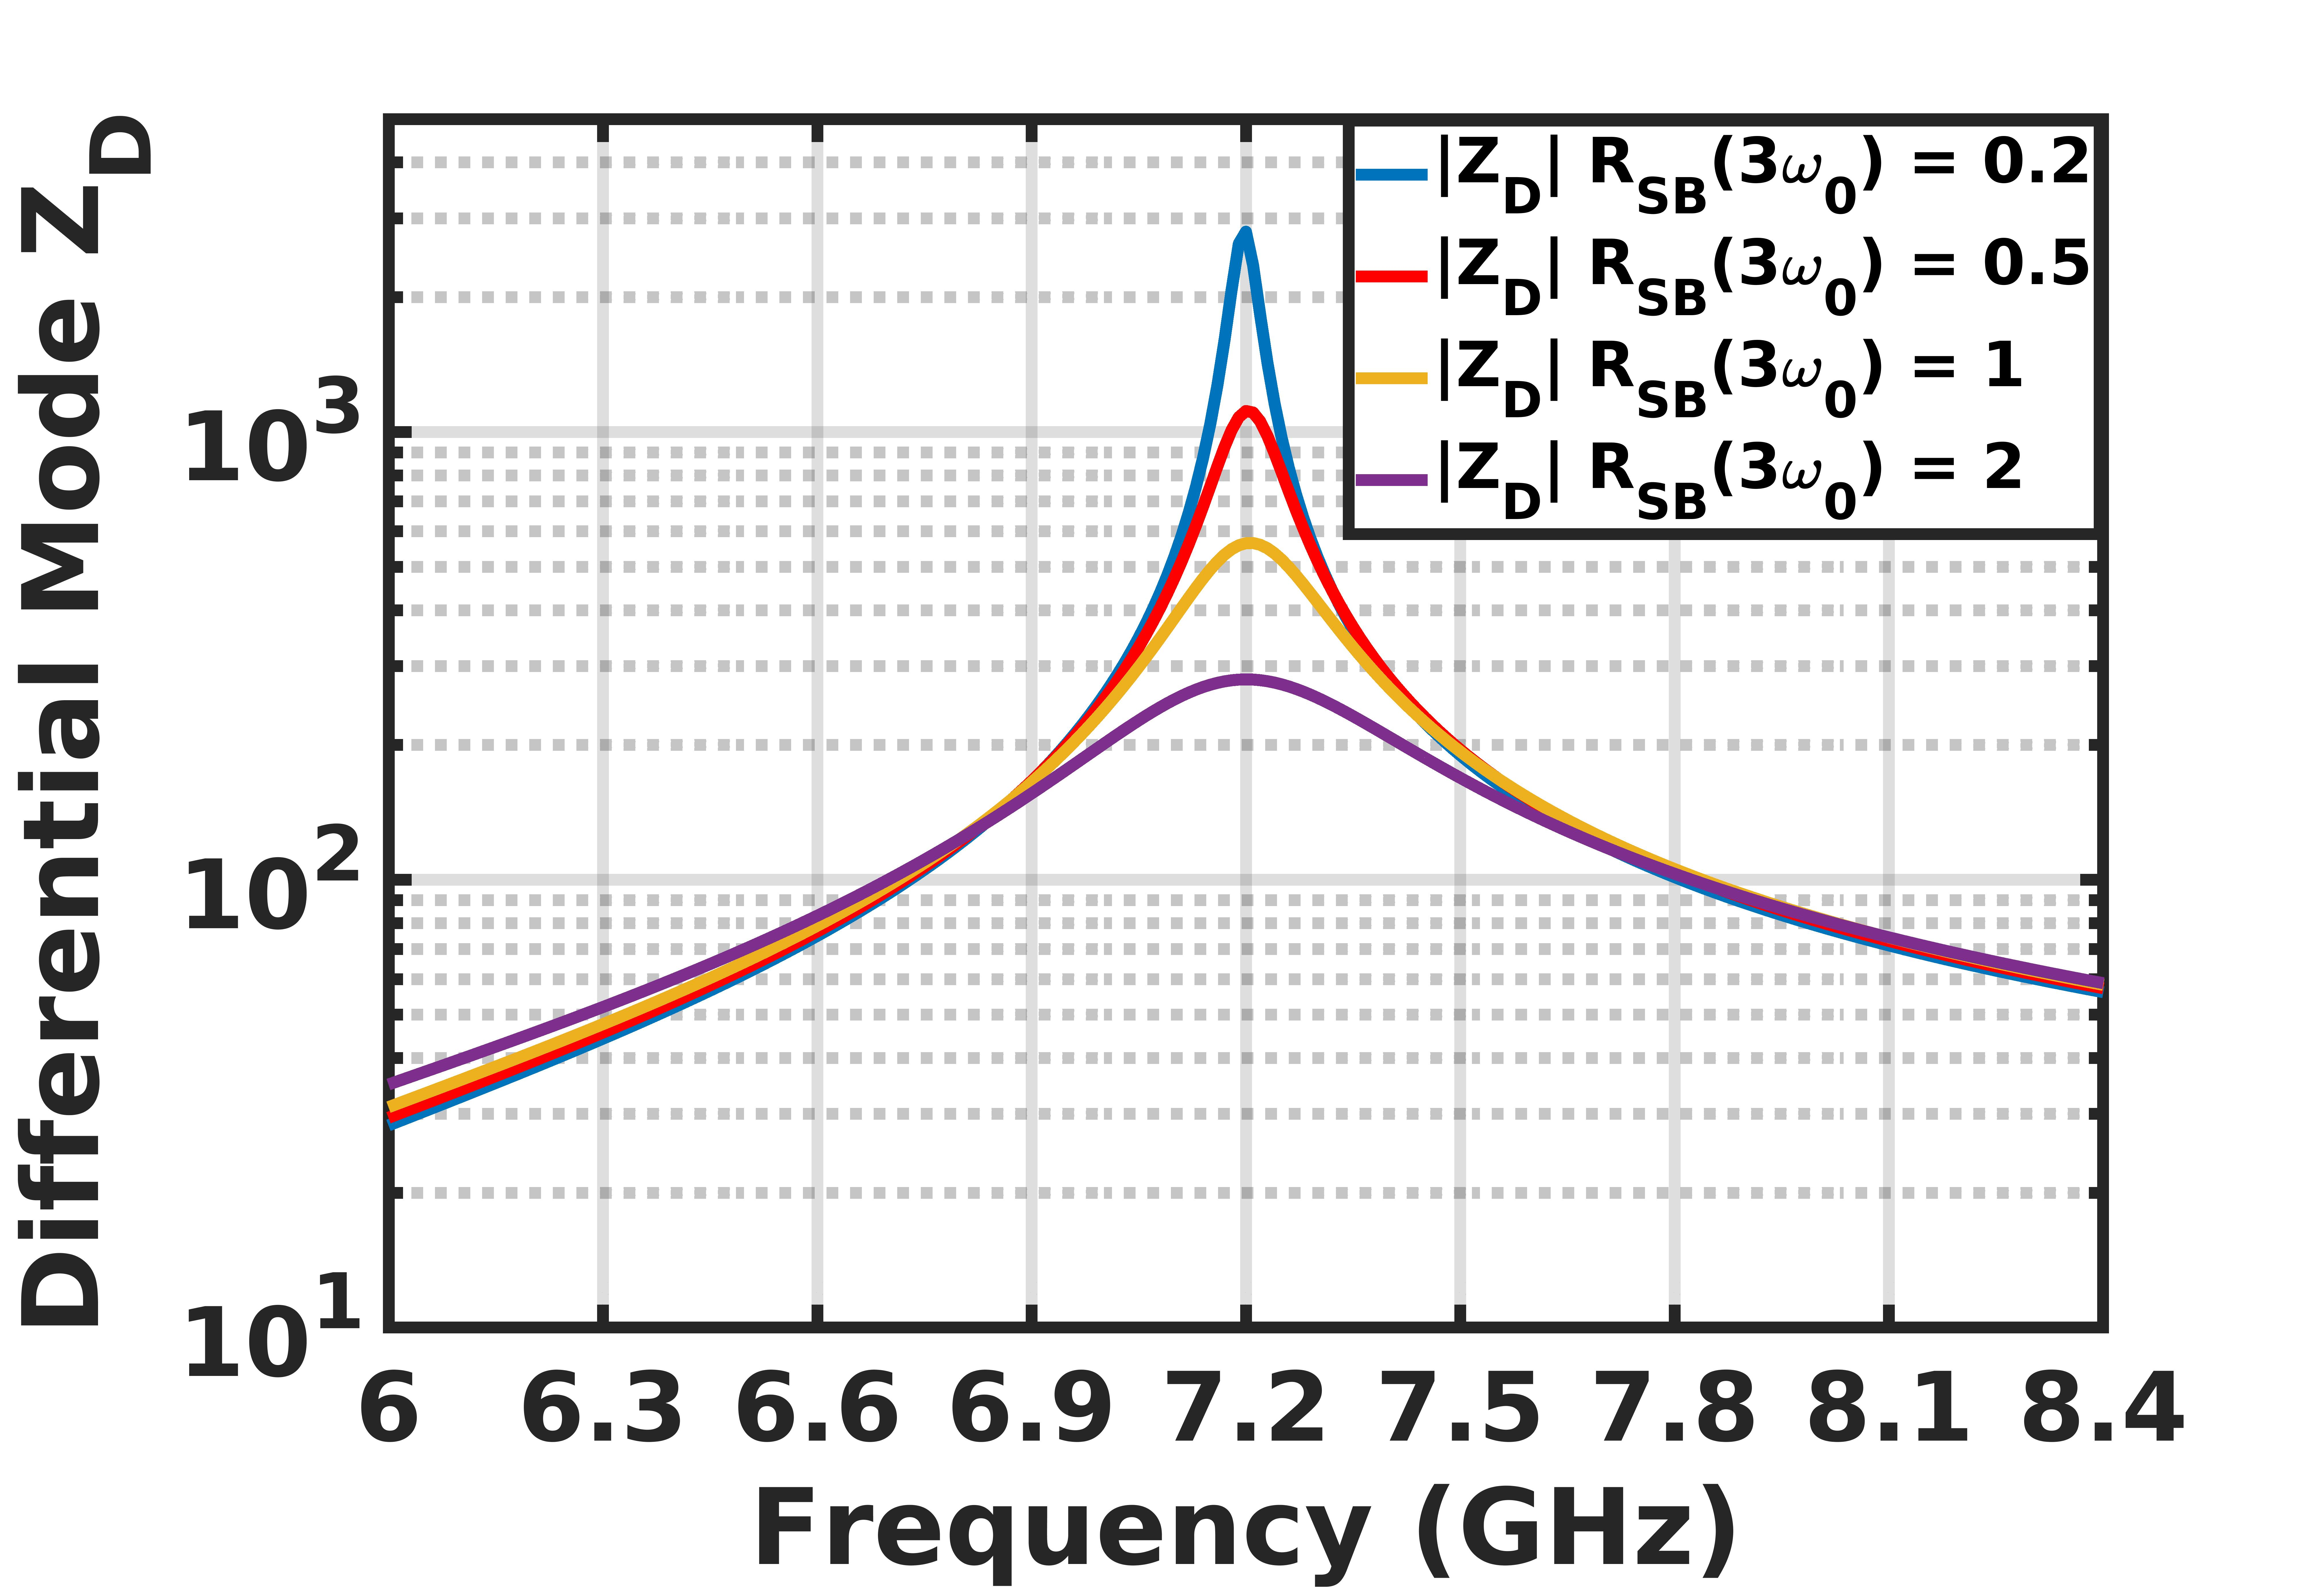
\includegraphics[width=1\textwidth]{Images/Design/Design_A_Rn_var_3H.jpg}
\caption{}
\label{fig:Design_A_Rn_var_3H}
\end{subfigure}
\begin{subfigure}{0.4\textwidth}
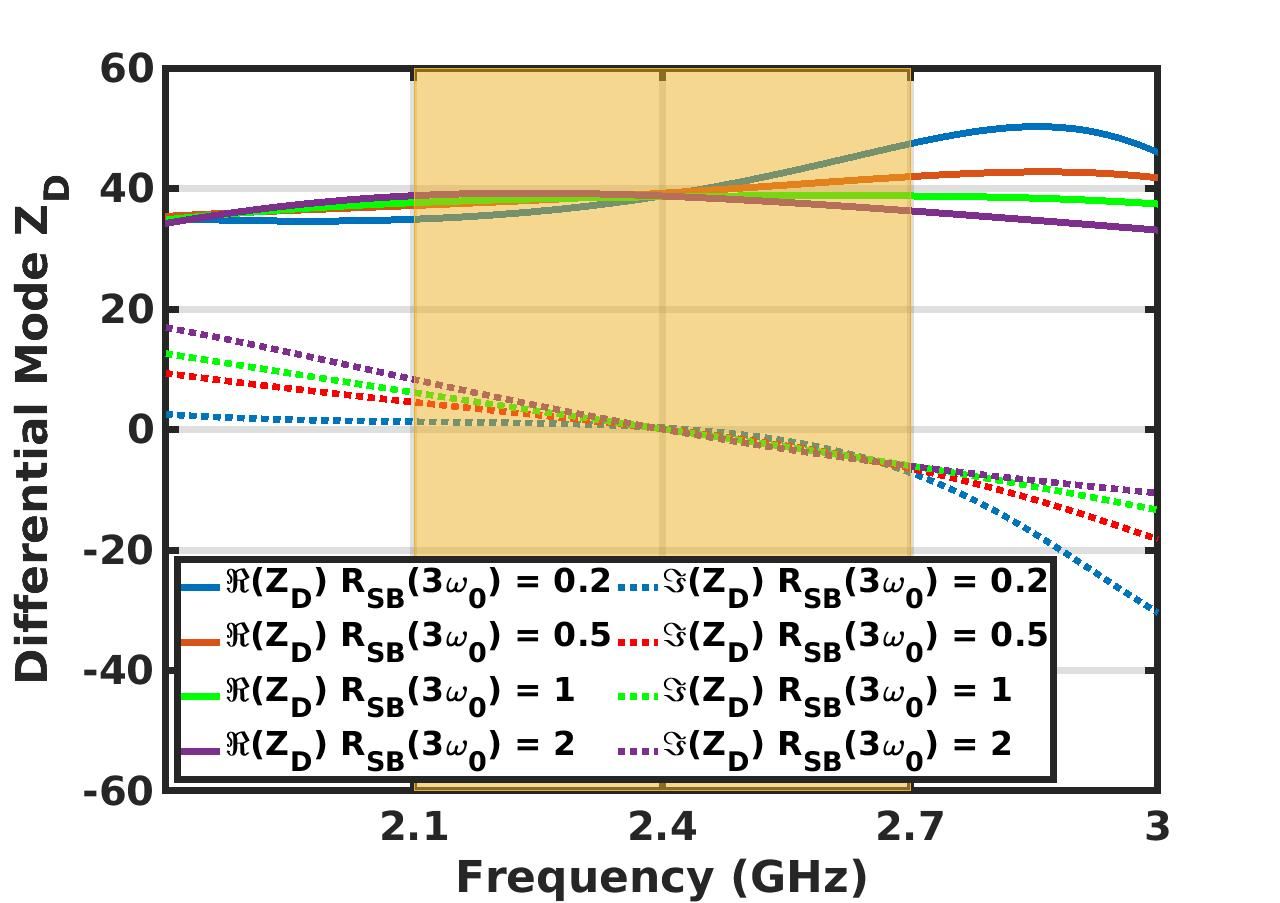
\includegraphics[width=1\textwidth]{Images/Design/Design_A_Rn_var_1H.jpg}
\caption{}
\label{fig:Design_A_Rn_var_1H}
\end{subfigure}
\caption{(a) Magnitude of $Z_{D}$ vs $\Re(Z_{SB})$ at $3\omega_0$; (b) Magnitude of $Z_D$ at $3^{rd}$ harmonic for different $R_{SB}(3\omega_0)$; (c) $Z_D$ at fundamental for different $R_{SB}(3\omega_0)$}
\label{fig:Design_A_Rn_var}
\end{figure}

The \textit{5} unknowns in the circuit: $km$, $N$, $L_P$, $C_2$, and $C_L$ can be calculated by assuming one of them and using \textit{4} equations ($\Re(Z_{SB})(\omega_0) =  29.8\hspace{1mm} \Omega$, $\Im(Z_{SB})(\omega_0) = 16.6\hspace{1mm}\Omega$, $\Re(Z_{SB})(3\omega_0) = 0.5\hspace{1mm}\Omega$ and  $\Im(Z_{SB})(3\omega_0) = 24.96\hspace{1mm}\Omega$). In this paper, $km =$ \textit{0.8} is assumed and the remaining unknowns ($N =$ \textit{1.34}, $L_P =$ \textit{2.2 nH}, $C_L =$ \textit{0.9 pF}, $C_2 =$ \textit{1.5 pF}, $L_2 =$ \textit{0.73 nH}) are calculated. The $km$ can be varied to get different sets of results in which $L_P$ is minimal and thereby making it layout friendly.


\subsection{Design B (no RF choke \& no $L_2C_2$)}

\begin{figure}[!t]
\captionsetup{font=footnotesize}
\centering
\begin{subfigure}{0.24\textwidth}
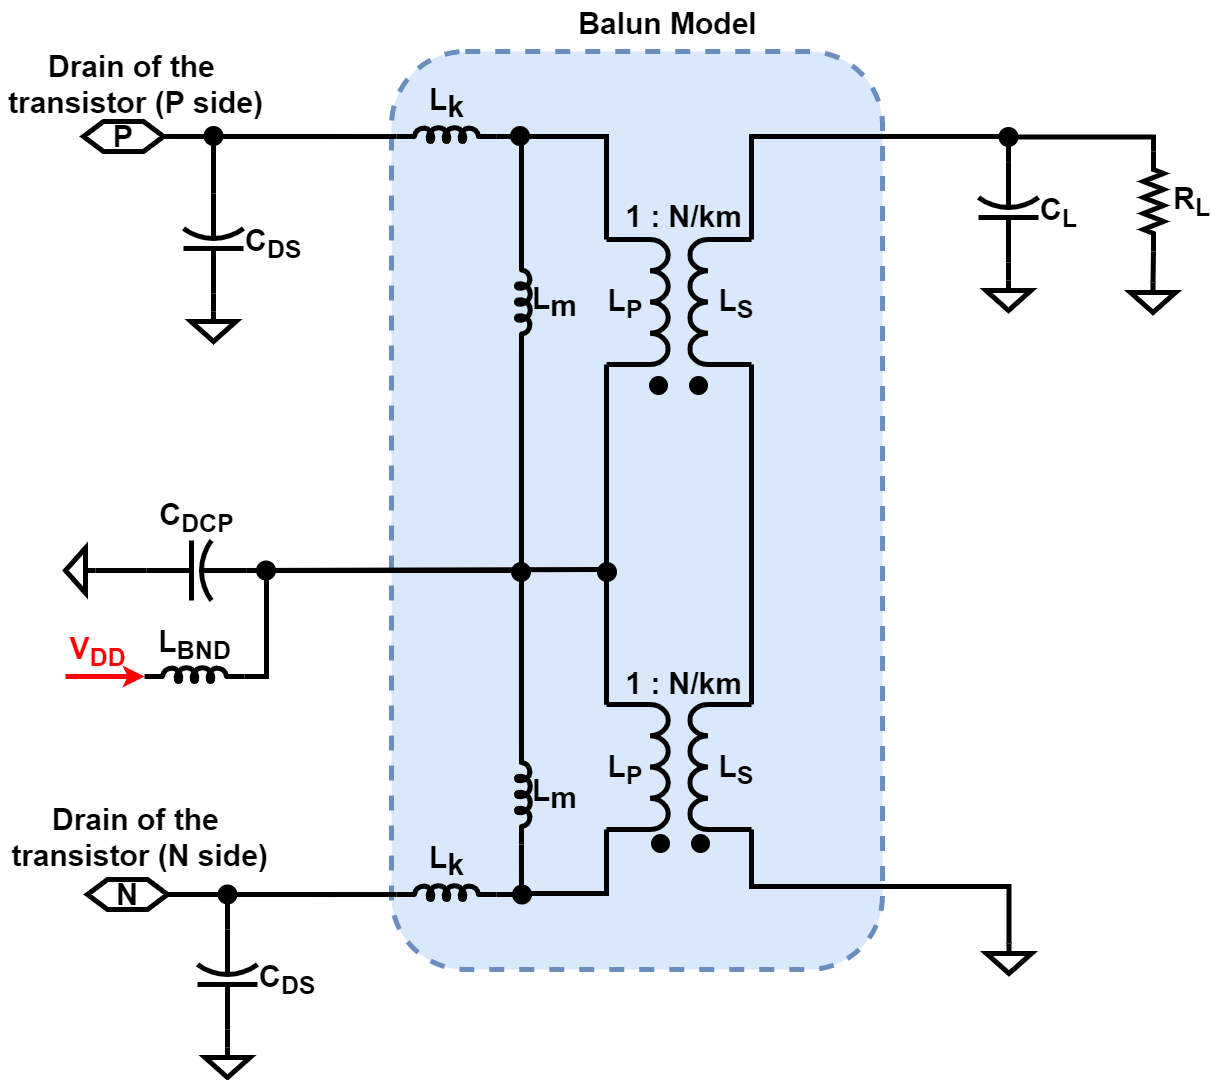
\includegraphics[width=1\textwidth]{Images/Design/Design_B_FC.png}
\caption{}
\label{fig:Design_B_FC}
\end{subfigure}
\begin{subfigure}{0.24\textwidth}
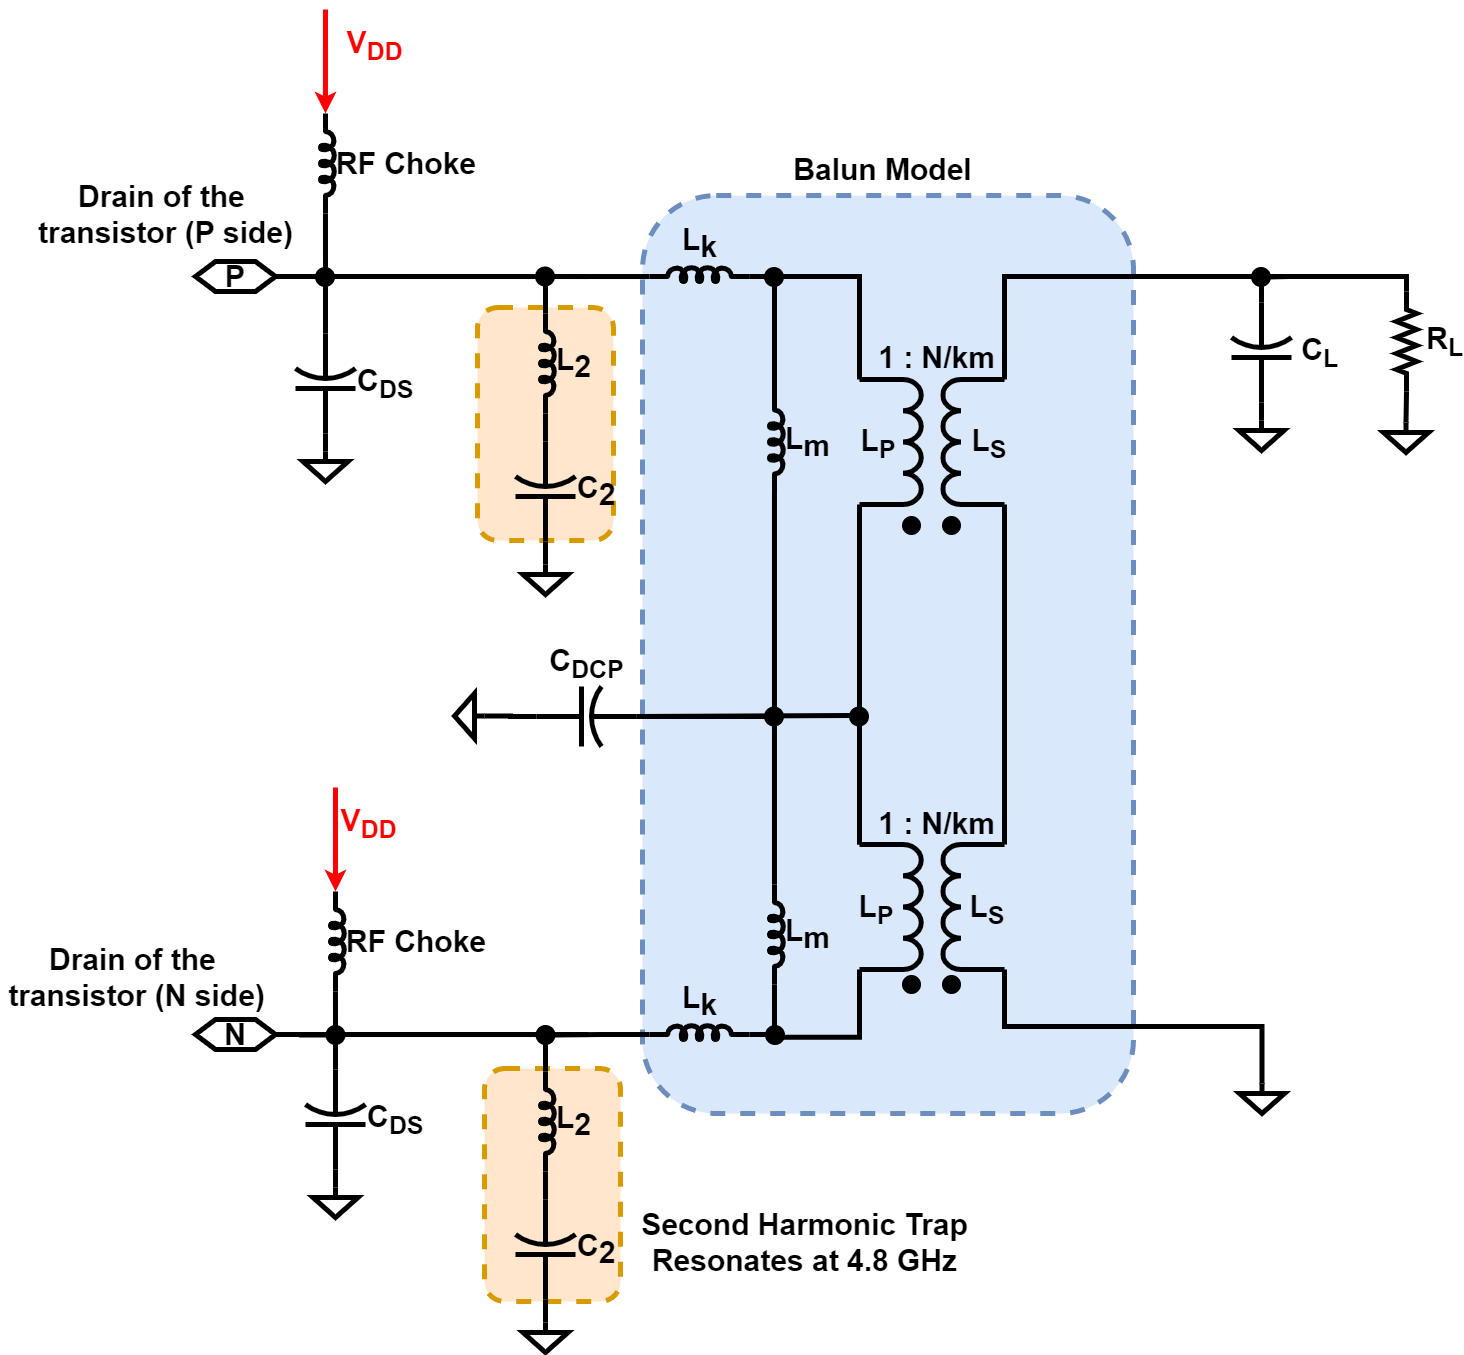
\includegraphics[width=1\textwidth]{Images/Design/Design_C_FC.png}
\caption{}
\label{fig:Design_C_FC}
\end{subfigure}
\begin{subfigure}{0.24\textwidth}
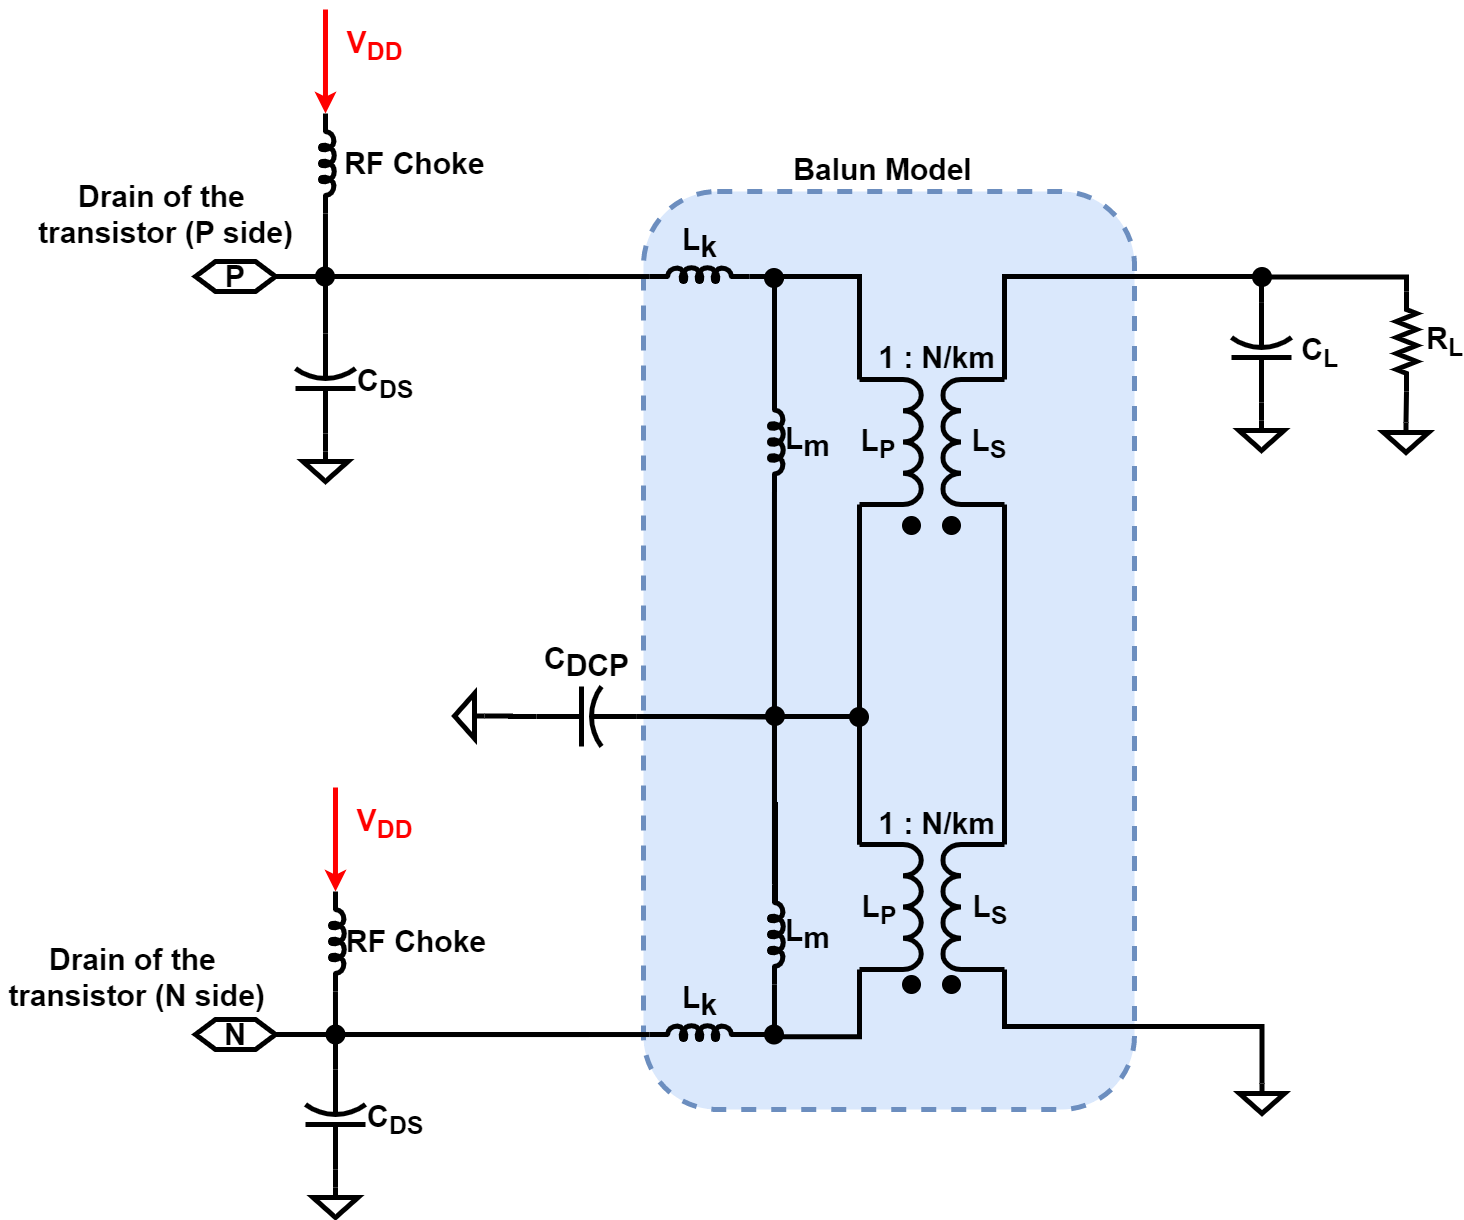
\includegraphics[width=1\textwidth]{Images/Design/Design_D_FC.png}
\caption{}
\label{fig:Design_D_FC}
\end{subfigure}
\caption{(a) Design B (Balun and $C_L$); (b) Design C (Balun, RF Choke, $L_2C_2$ \& $C_L$); (c) Design D (Balun, RF Choke \& $C_L$)}
\label{fig:Design_B_C_D}
\end{figure}

In this design (Figure \ref{fig:Design_B_FC}), $L_2C_2$ is removed so it reduces the number of unknowns. Like the previous case, differential mode analysis yields \textit{4} equations and there are \textit{4} unknowns, thus leading to a single set of values for $km =$ \textit{0.72}, $N =$ \textit{0.9}, $L_P =$ \textit{0.63 nH}, $C_L =$ \textit{3.96 pF}, unlike design A. $C_{DCP}$ is tuned to provide a short at $2\omega_0$ such that $C_{DCP}$ resonates with $L_P$, $L_{BND}$ and $C_{DS}$ which is obtained from the common mode analysis. Moreover, $C_{DCP}$ provides RF ground and blocks DC.

\subsection{Design C (with RF choke \& with $L_2C_2$)}
In this design (Figure \ref{fig:Design_C_FC}), $V_{DD}$ is supplied through RF choke unlike the previous designs. RF chokes are assumed to have a fixed value of \textit{5 nH}. The differential mode analysis yields \textit{4} equations similar to design A. Assuming $km =$ \textit{0.8}, the other unknowns are calculated as $N =$ \textit{1.14}, $L_P =$ \textit{2.23 nH}, $C_L =$ \textit{1.10 pF}, $C_2 =$ \textit{1.37 pF}.
Like design A, $C_2$ should resonate out with $L_2$ to get short at $2\omega_0$. Thus, $L_2 =$ \textit{0.8 nH}. 

\subsection{Design D (with RF choke \& no $L_2C_2$)}
 Unlike design C, $L_2C_2$ is removed in this design (Figure \ref{fig:Design_D_FC}). Also, RF choke should be calculated assuming $C_{DS}$ resonates with it at $\omega_0$ (RF Choke = \textit{2.35 nH}).
The differential mode analysis yields \textit{4} equations and the \textit{4} unknowns ($N =$ \textit{0.84}, $L_P =$ \textit{0.86 nH}, $C_L =$ \textit{3.95 pF}, $km =$ \textit{0.77}) can be calculated.
$C_{DCP}$ can be tuned to provide a short at $2\omega_0$.

\section{Results}
\label{section:Results}

Figures \ref{fig:Comp_1H} and \ref{fig:Comp_2H_imag}  show that all the \textit{4} designs satisfying the main CCF requirements which is decreasing trend of the reactive part at fundamental and increasing trend of the reactive part at $2^{nd}$ harmonic.
From Figure \ref{fig:Comp_1H}, it is seen that the real part at fundamental is flatter in the bandwidth \textit{2.1 - 2.7 GHz} for design A and C which, in turn, leads to constant $P_{OUT}$ in the specified bandwidth unlike design B and D. The $L_2C_2$ which acts as a varying capacitor at fundamental hold the reason for this. The designs B and D have a higher reactive part at the fundamental as compared to other designs which in turn leads to larger $\gamma$ value (refer equation \ref{eqn_CCF_imp}) and thus, higher peak factor (refer Figure \ref{fig:CCF_wave_VI}). Figures \ref{fig:Comp_2H_imag} and \ref{fig:Comp_3H_Mag} show that all the \textit{4} designs have similar response at $2^{nd}$ and $3^{rd}$ harmonic. 
%The impedance at \textit{2.1 GHz} and \textit{2.7 GHz} is less than \textit{200} $\Omega$ for all the \textit{4} designs.

\begin{figure}[!t]
\captionsetup{font=footnotesize}
\centering
\begin{subfigure}{0.5\textwidth}
\centering
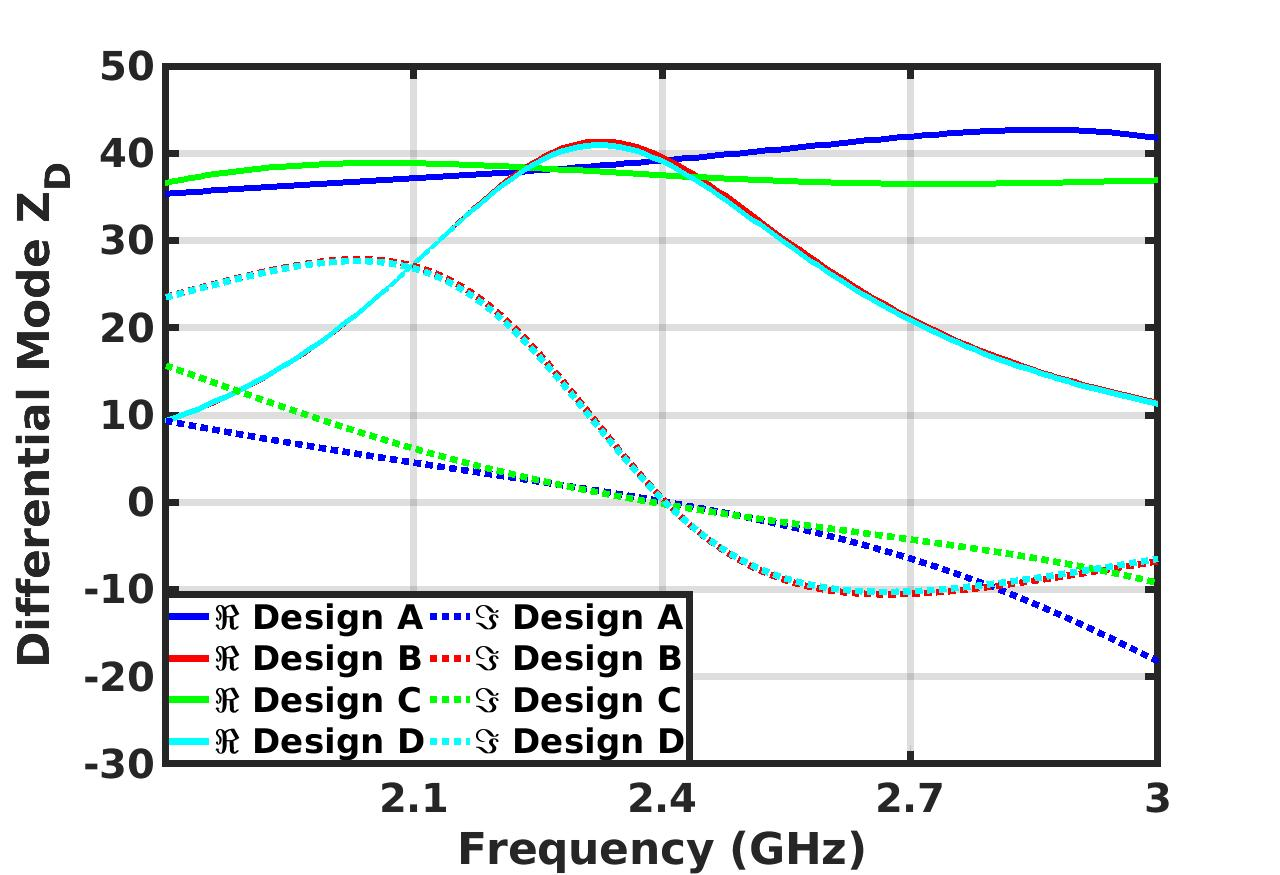
\includegraphics[width=0.65\textwidth]{Images/Output_Network_Comp/Comp_1H.jpg}
\caption{}
\label{fig:Comp_1H}
\end{subfigure}
\begin{subfigure}{0.24\textwidth}
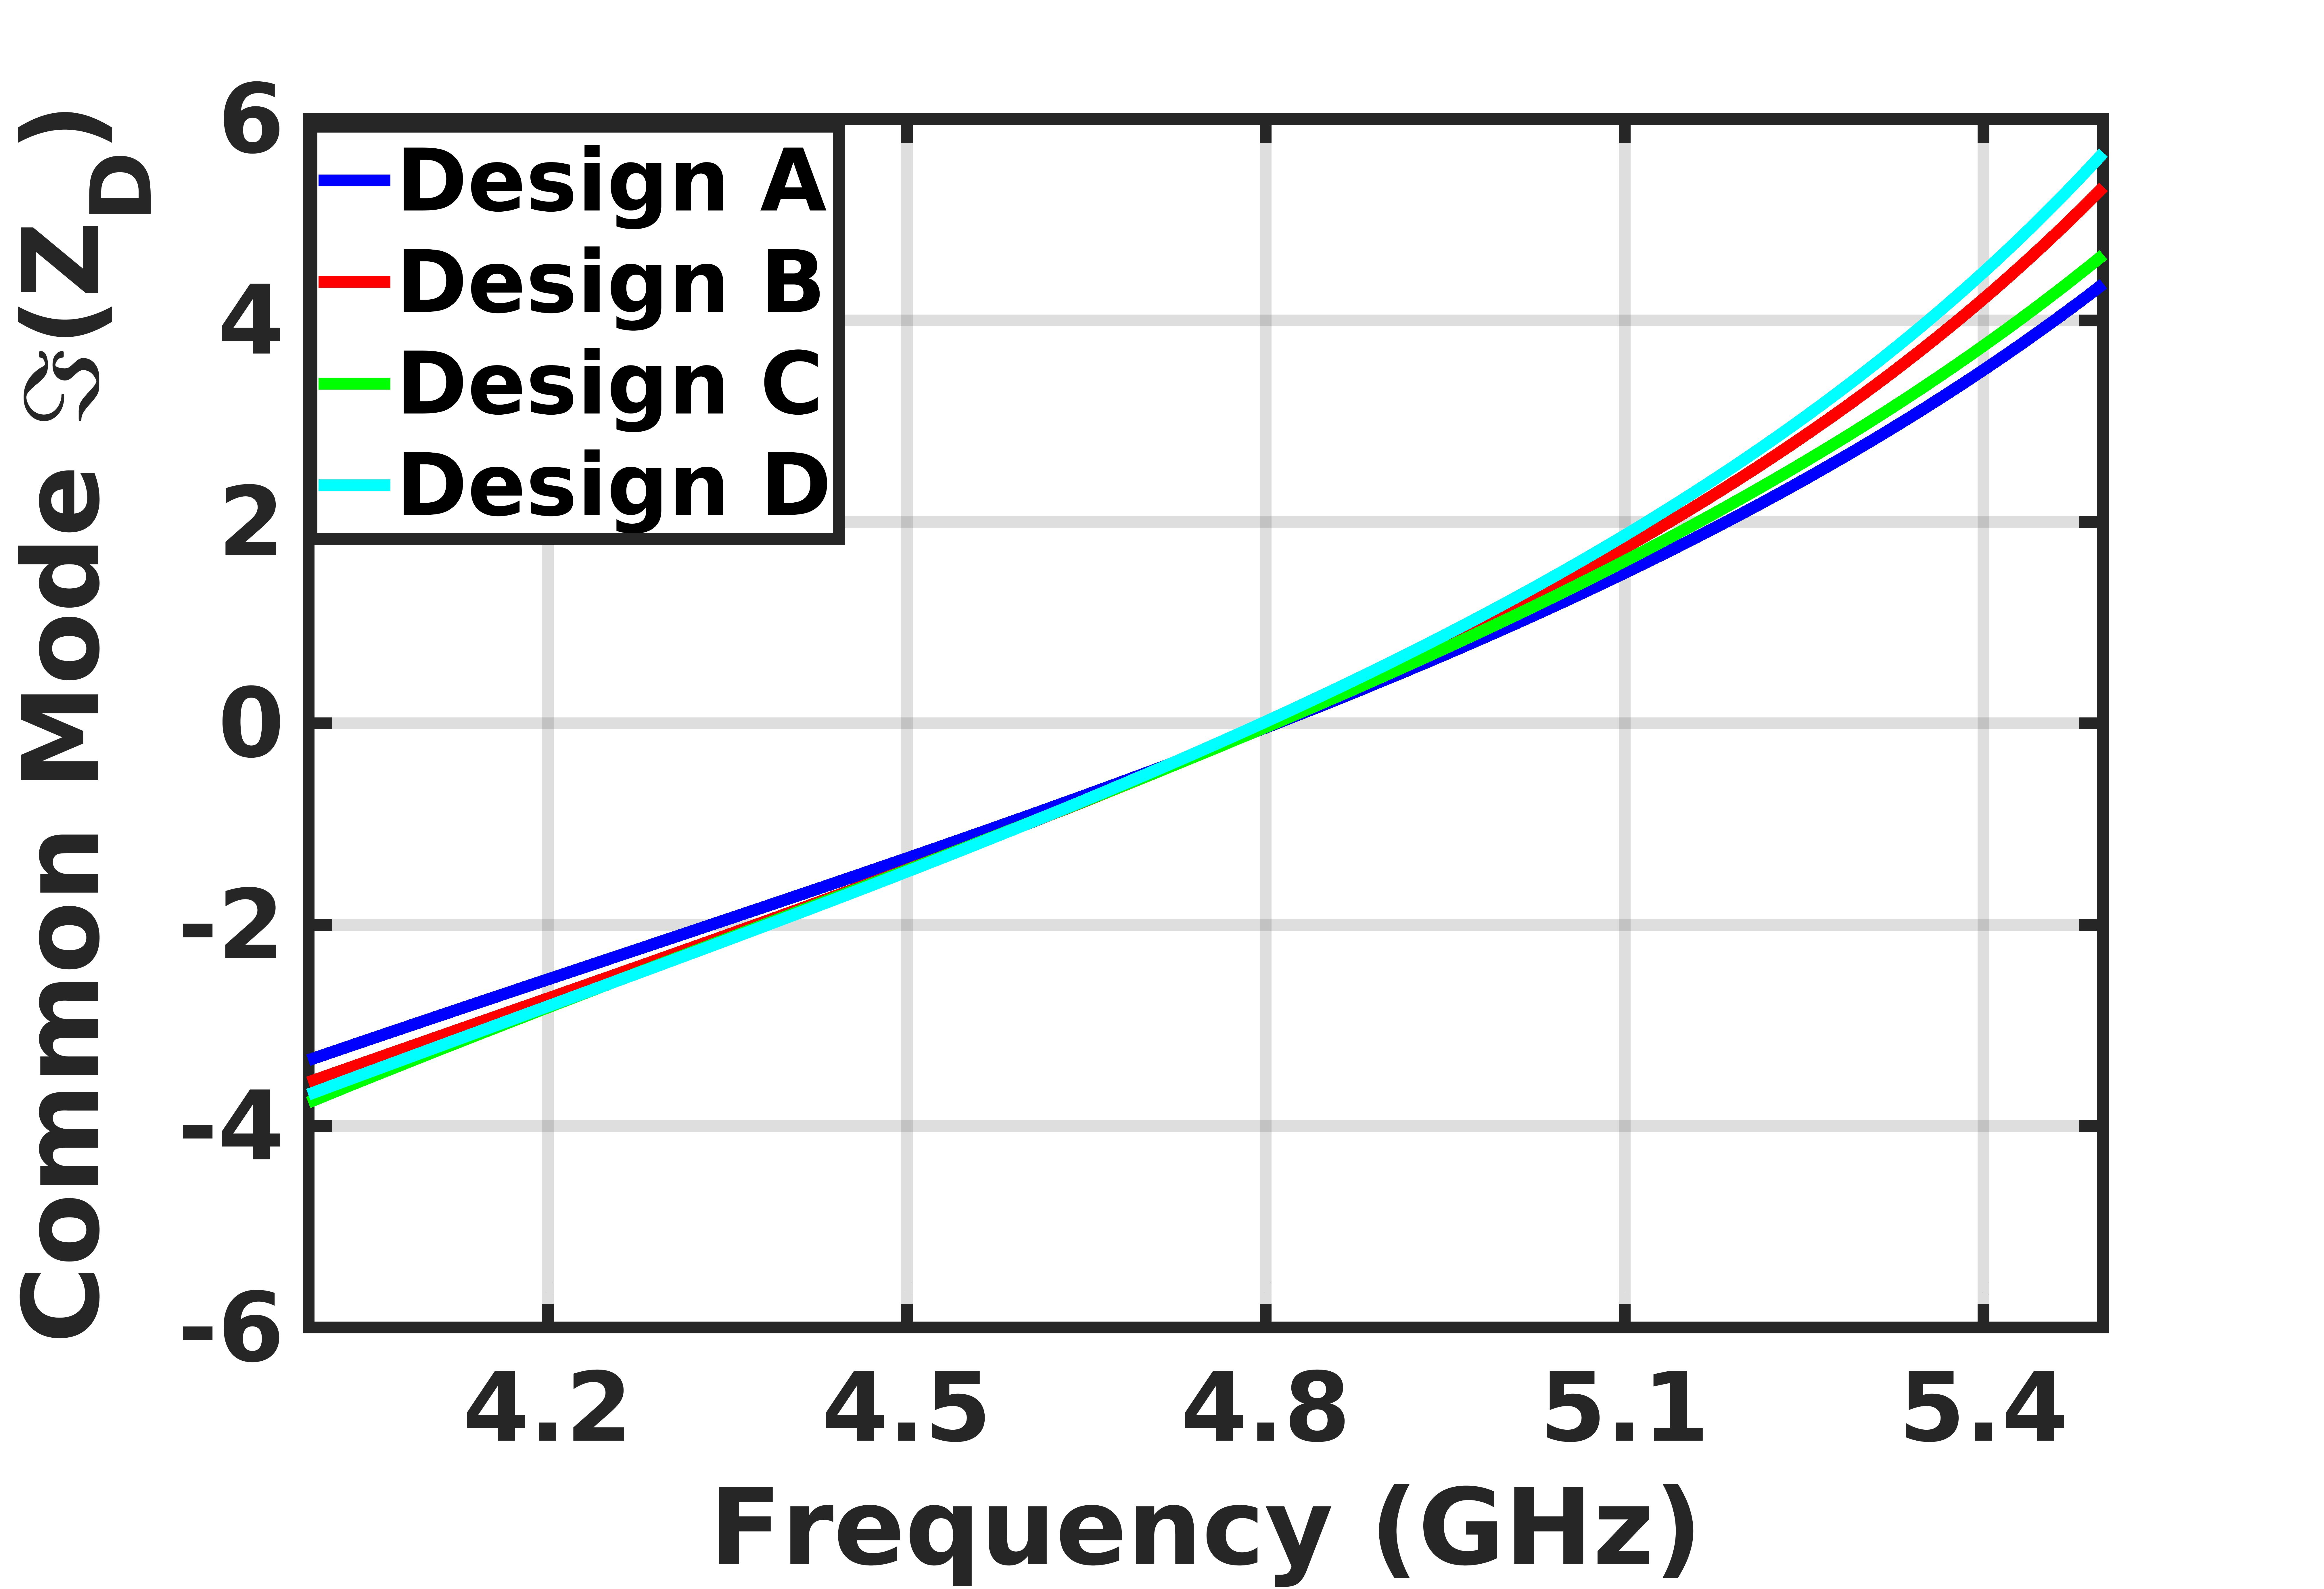
\includegraphics[width=1\textwidth]{Images/Output_Network_Comp/Comp_2H_imag.jpg}
\caption{}
\label{fig:Comp_2H_imag}
\end{subfigure}
\begin{subfigure}{0.24\textwidth}
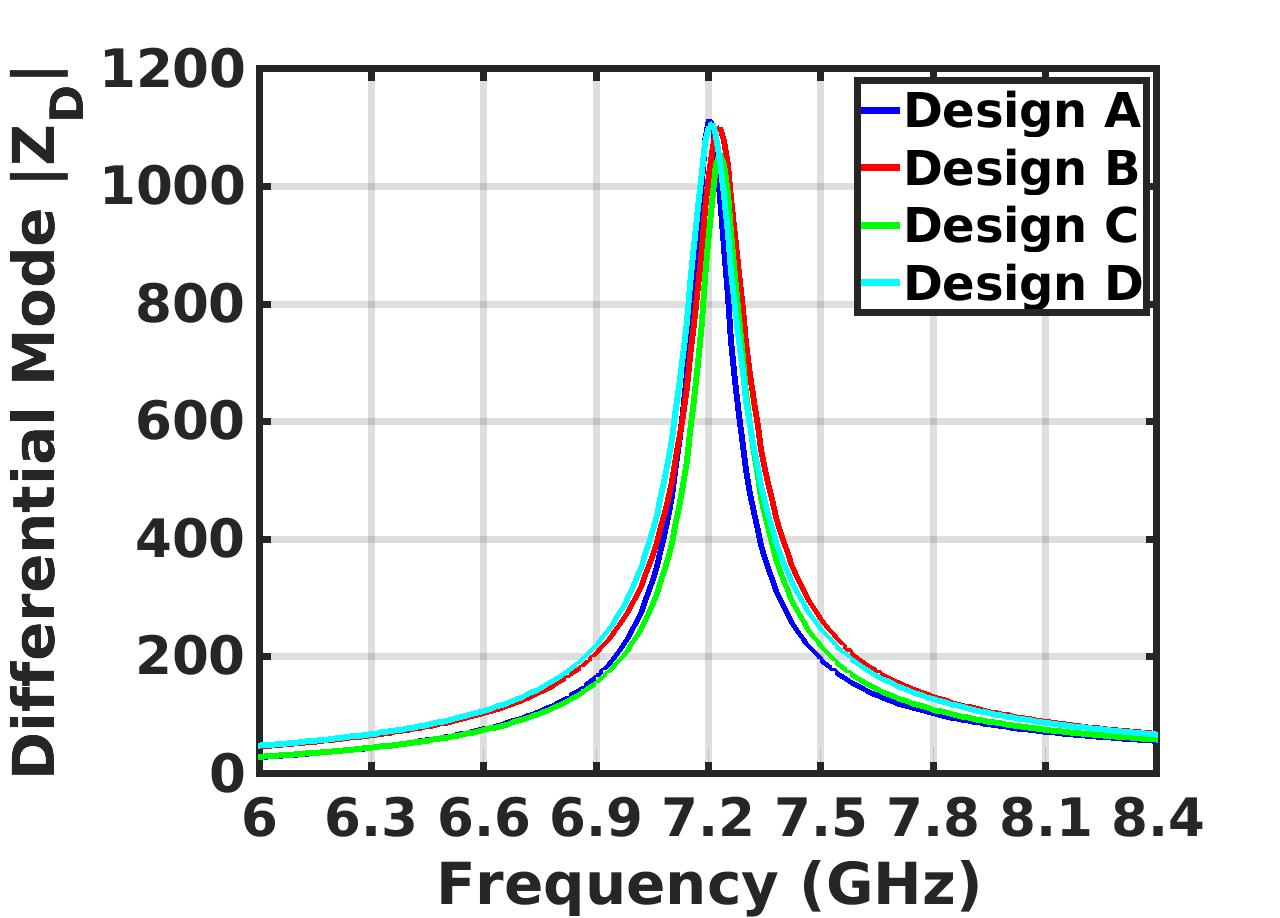
\includegraphics[width=1\textwidth]{Images/Output_Network_Comp/Comp_3H_Mag.jpg}
\caption{}
\label{fig:Comp_3H_Mag}
\end{subfigure}
\caption{(a) Impedance ($Z_D$) at $1^{st}$ harmonic; (b) Reactive part of $Z_D$ ($\Im(Z_D)$) at $2^{nd}$ harmonic; (c) Magnitude of $Z_D$ ($|Z_D|$) at $3^{rd}$ harmonic}
\label{fig:Comp_1H_2H_3H}
\vspace{-0.1in}
\end{figure}

%\begin{figure}[ht]
%\captionsetup{font=normalsize}
%\centering
%\begin{subfigure}{0.49\textwidth}
%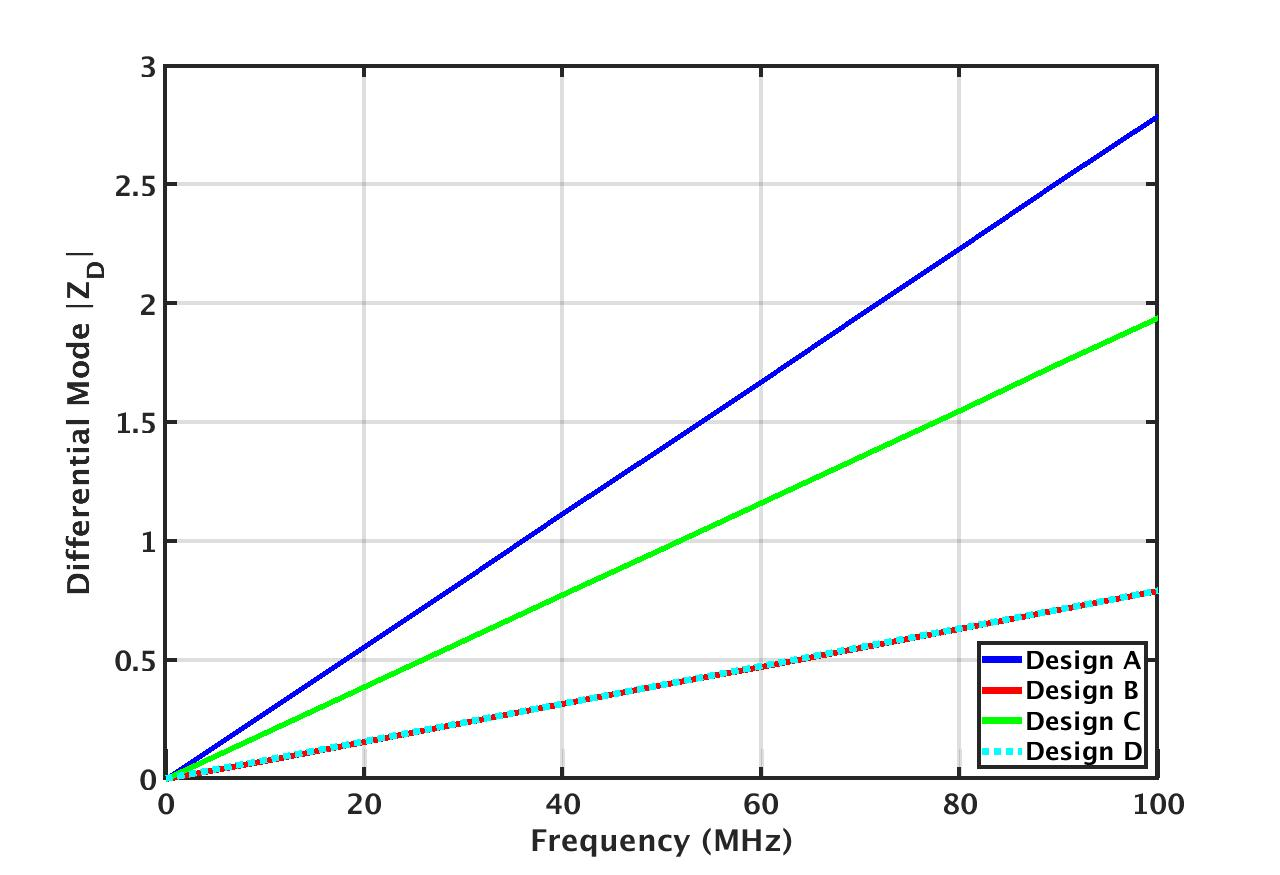
\includegraphics[width=1\linewidth, height=5cm]{Images/Output_Network_Comp/Comp_Diff_Lf.jpg} \caption{Differential mode impedance}
%\label{fig:Comp_Diff_Lf}
%\end{subfigure}
%\begin{subfigure}{0.49\textwidth}
%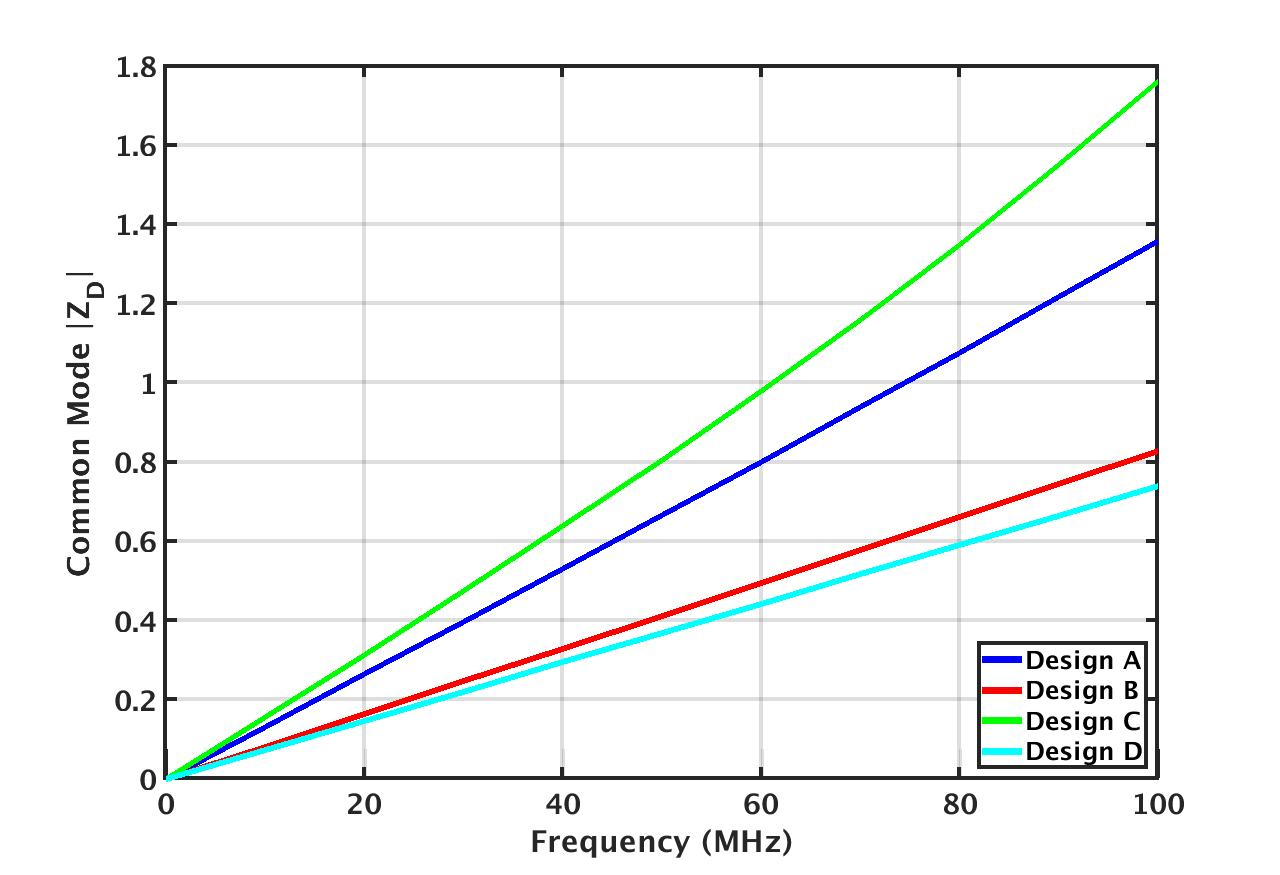
\includegraphics[width=1\linewidth, height=5cm]{Images/Output_Network_Comp/Comp_Com_Lf.jpg}
%\caption{Common mode impedance}
%\label{fig:Comp_Com_Lf}
%\end{subfigure}
%\caption{Impedance at low frequency}
%\label{fig:Comp_Lf}
%\end{figure}

%\ref{fig:Comp_Diff_Lf} and \ref{fig:Comp_Com_Lf} shows that differential and common mode impedance isn't large (less than \textit{4} $\Omega$) between \textit{0 - 100 MHz}. In case, the impedance was large, it can reduce third order intercept point ($IP_3$) due to indirect mixing \cite{Baseband_Impedance_IM3_1} \cite{Baseband_Impedance_IM3_2} \cite{Baseband_Impedance_IM3_3}.  
%The impedance at \textit{2.1 GHz} and \textit{2.7 GHz} is less than \textit{200} $\Omega$ for all the \textit{4} designs
The \textit{4} output networks are tested with an ideal output stage (single transistor which acts as a current source when turned on) in ADS. Figure \ref{fig:Comp_Pout_DE} shows there is a large variation in peak $P_{OUT}$ and maximum $\eta_D$ across the operational bandwidth for the design B and D, unlike design A and C. This variation can be attributed to the varying real part at the fundamental in those designs.
So from the simulation, it is seen that design A outperforms other designs since it has the least number of components as well as more constant $P_{\text{OUT}}$ and $\eta_D$ in the specified bandwidth.

\begin{figure}[!t]
\captionsetup{font=footnotesize}
\centering
\begin{subfigure}{0.24\textwidth}
\centering
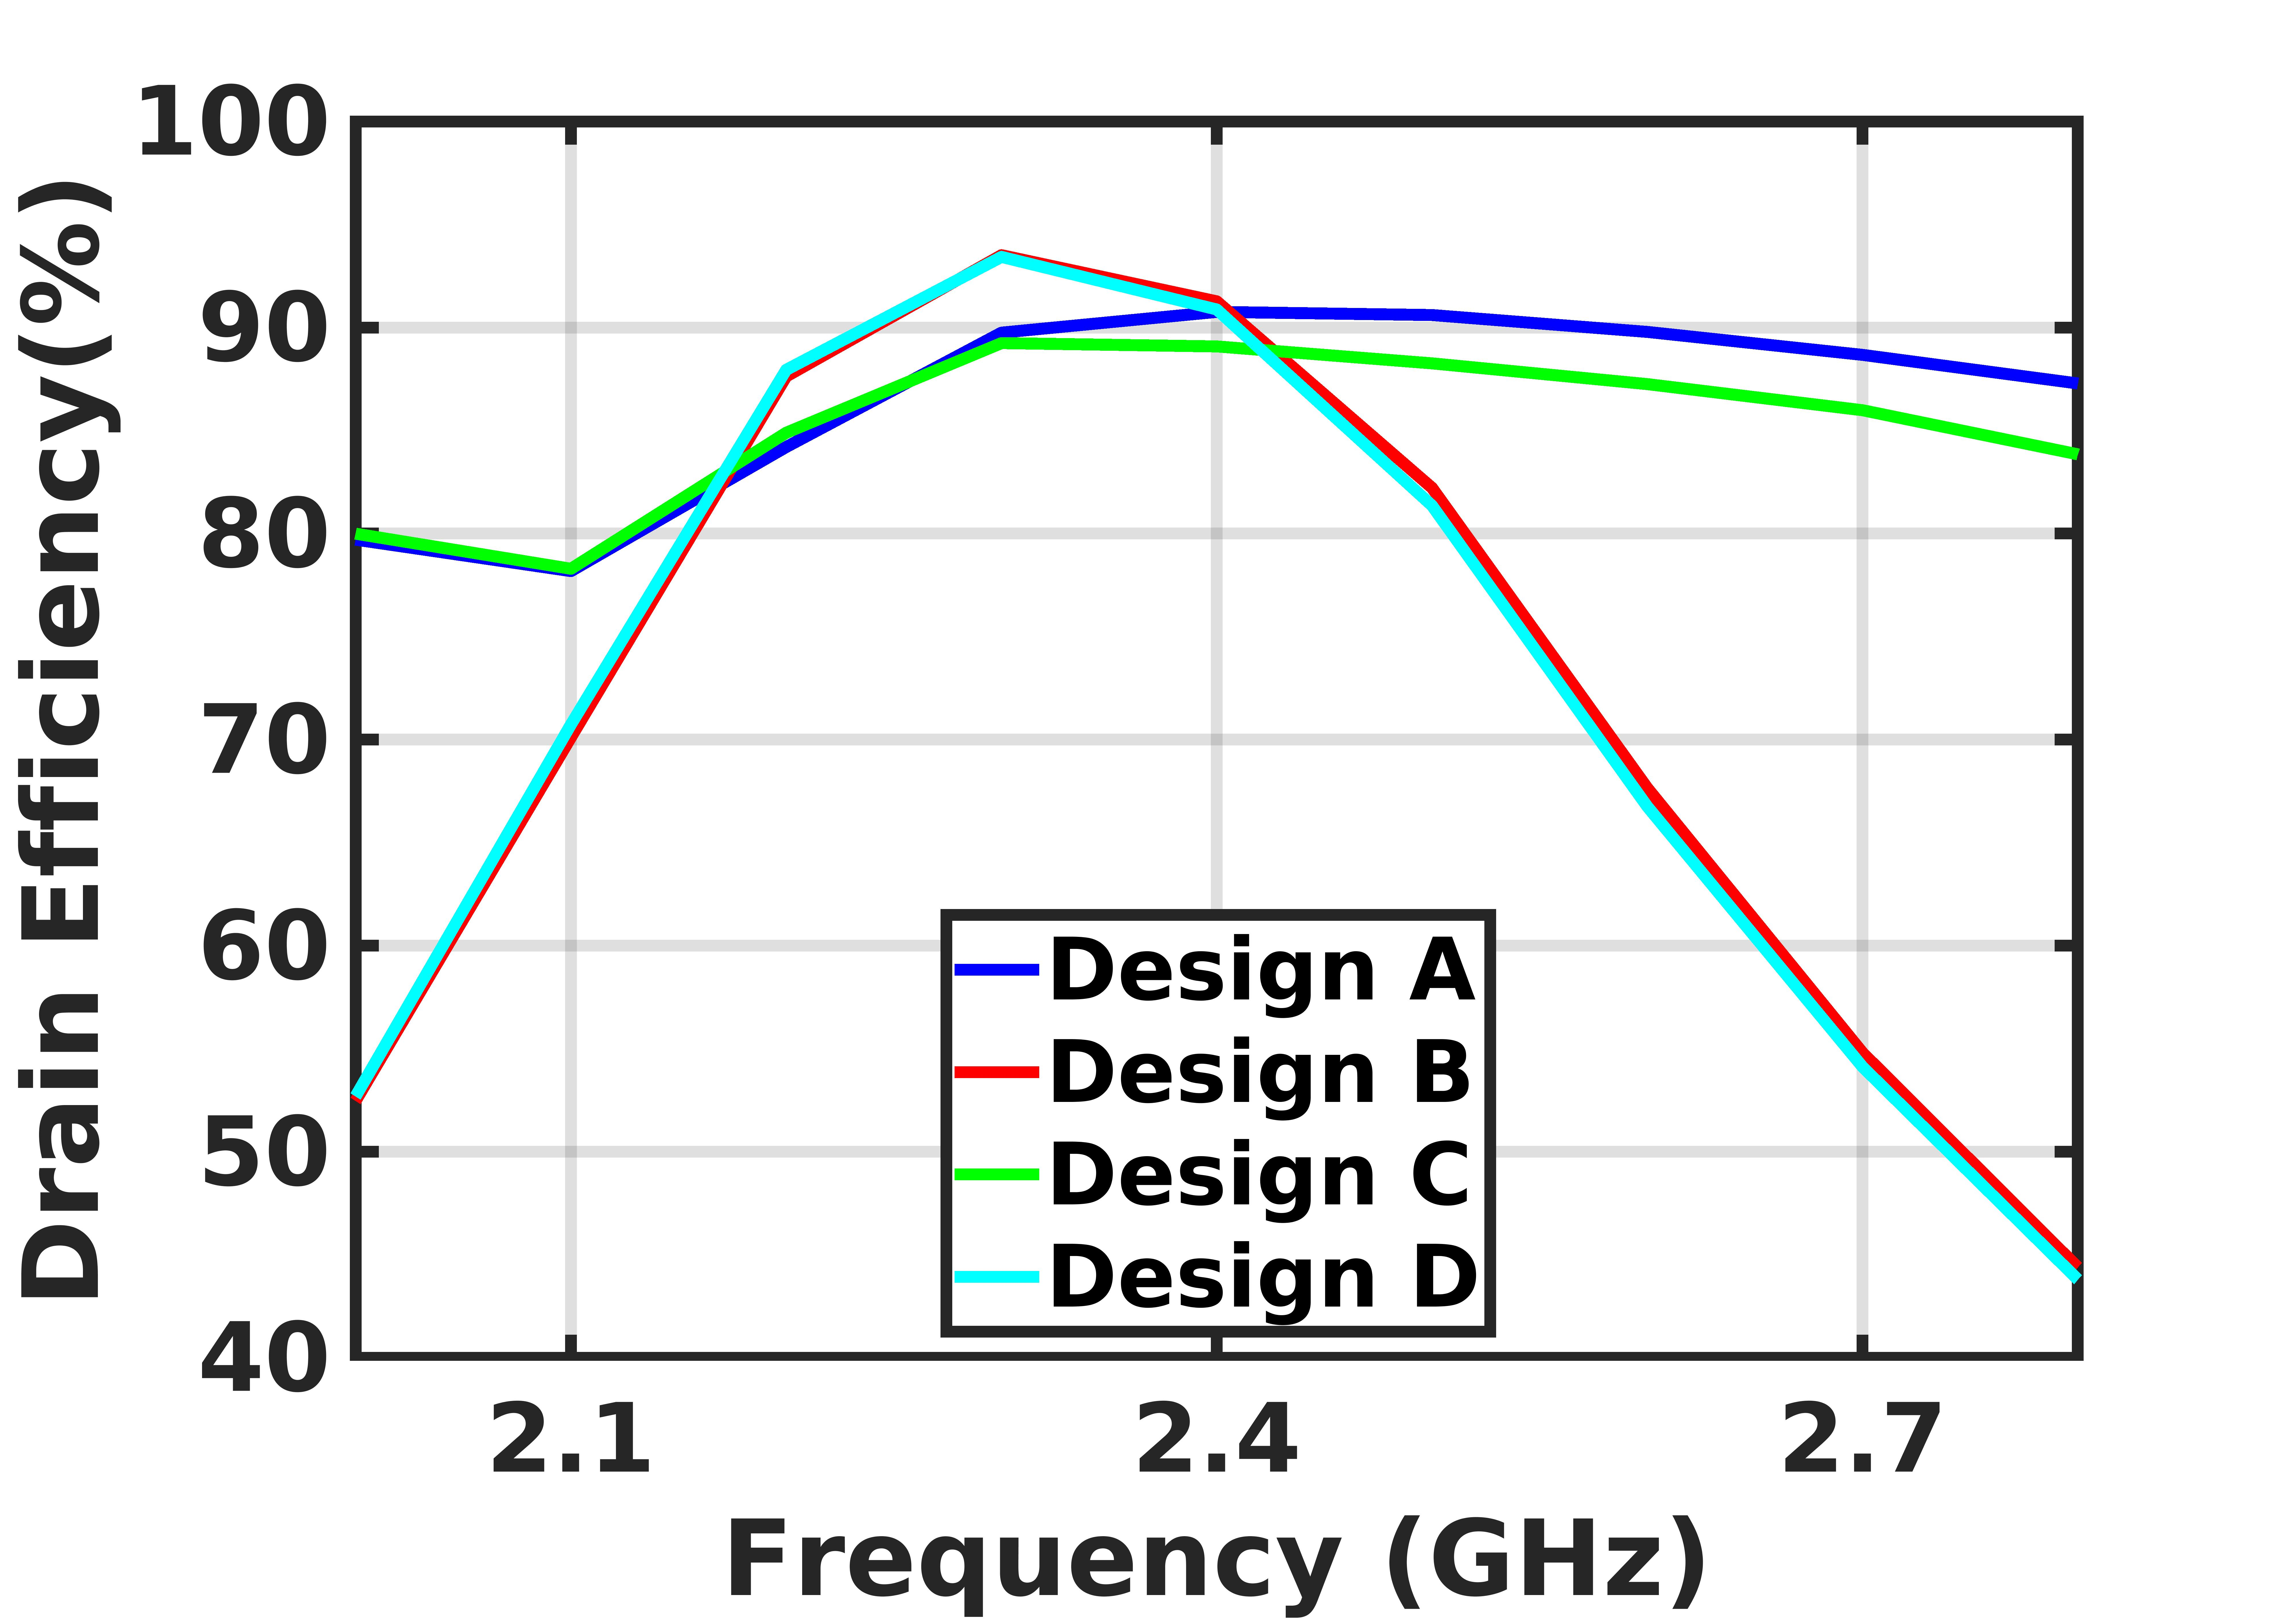
\includegraphics[width=1\textwidth]{Images/Output_Network_Comp/Comp_DE.jpg}
\caption{}
\label{fig:Comp_DE}
\end{subfigure}
\begin{subfigure}{0.24\textwidth}
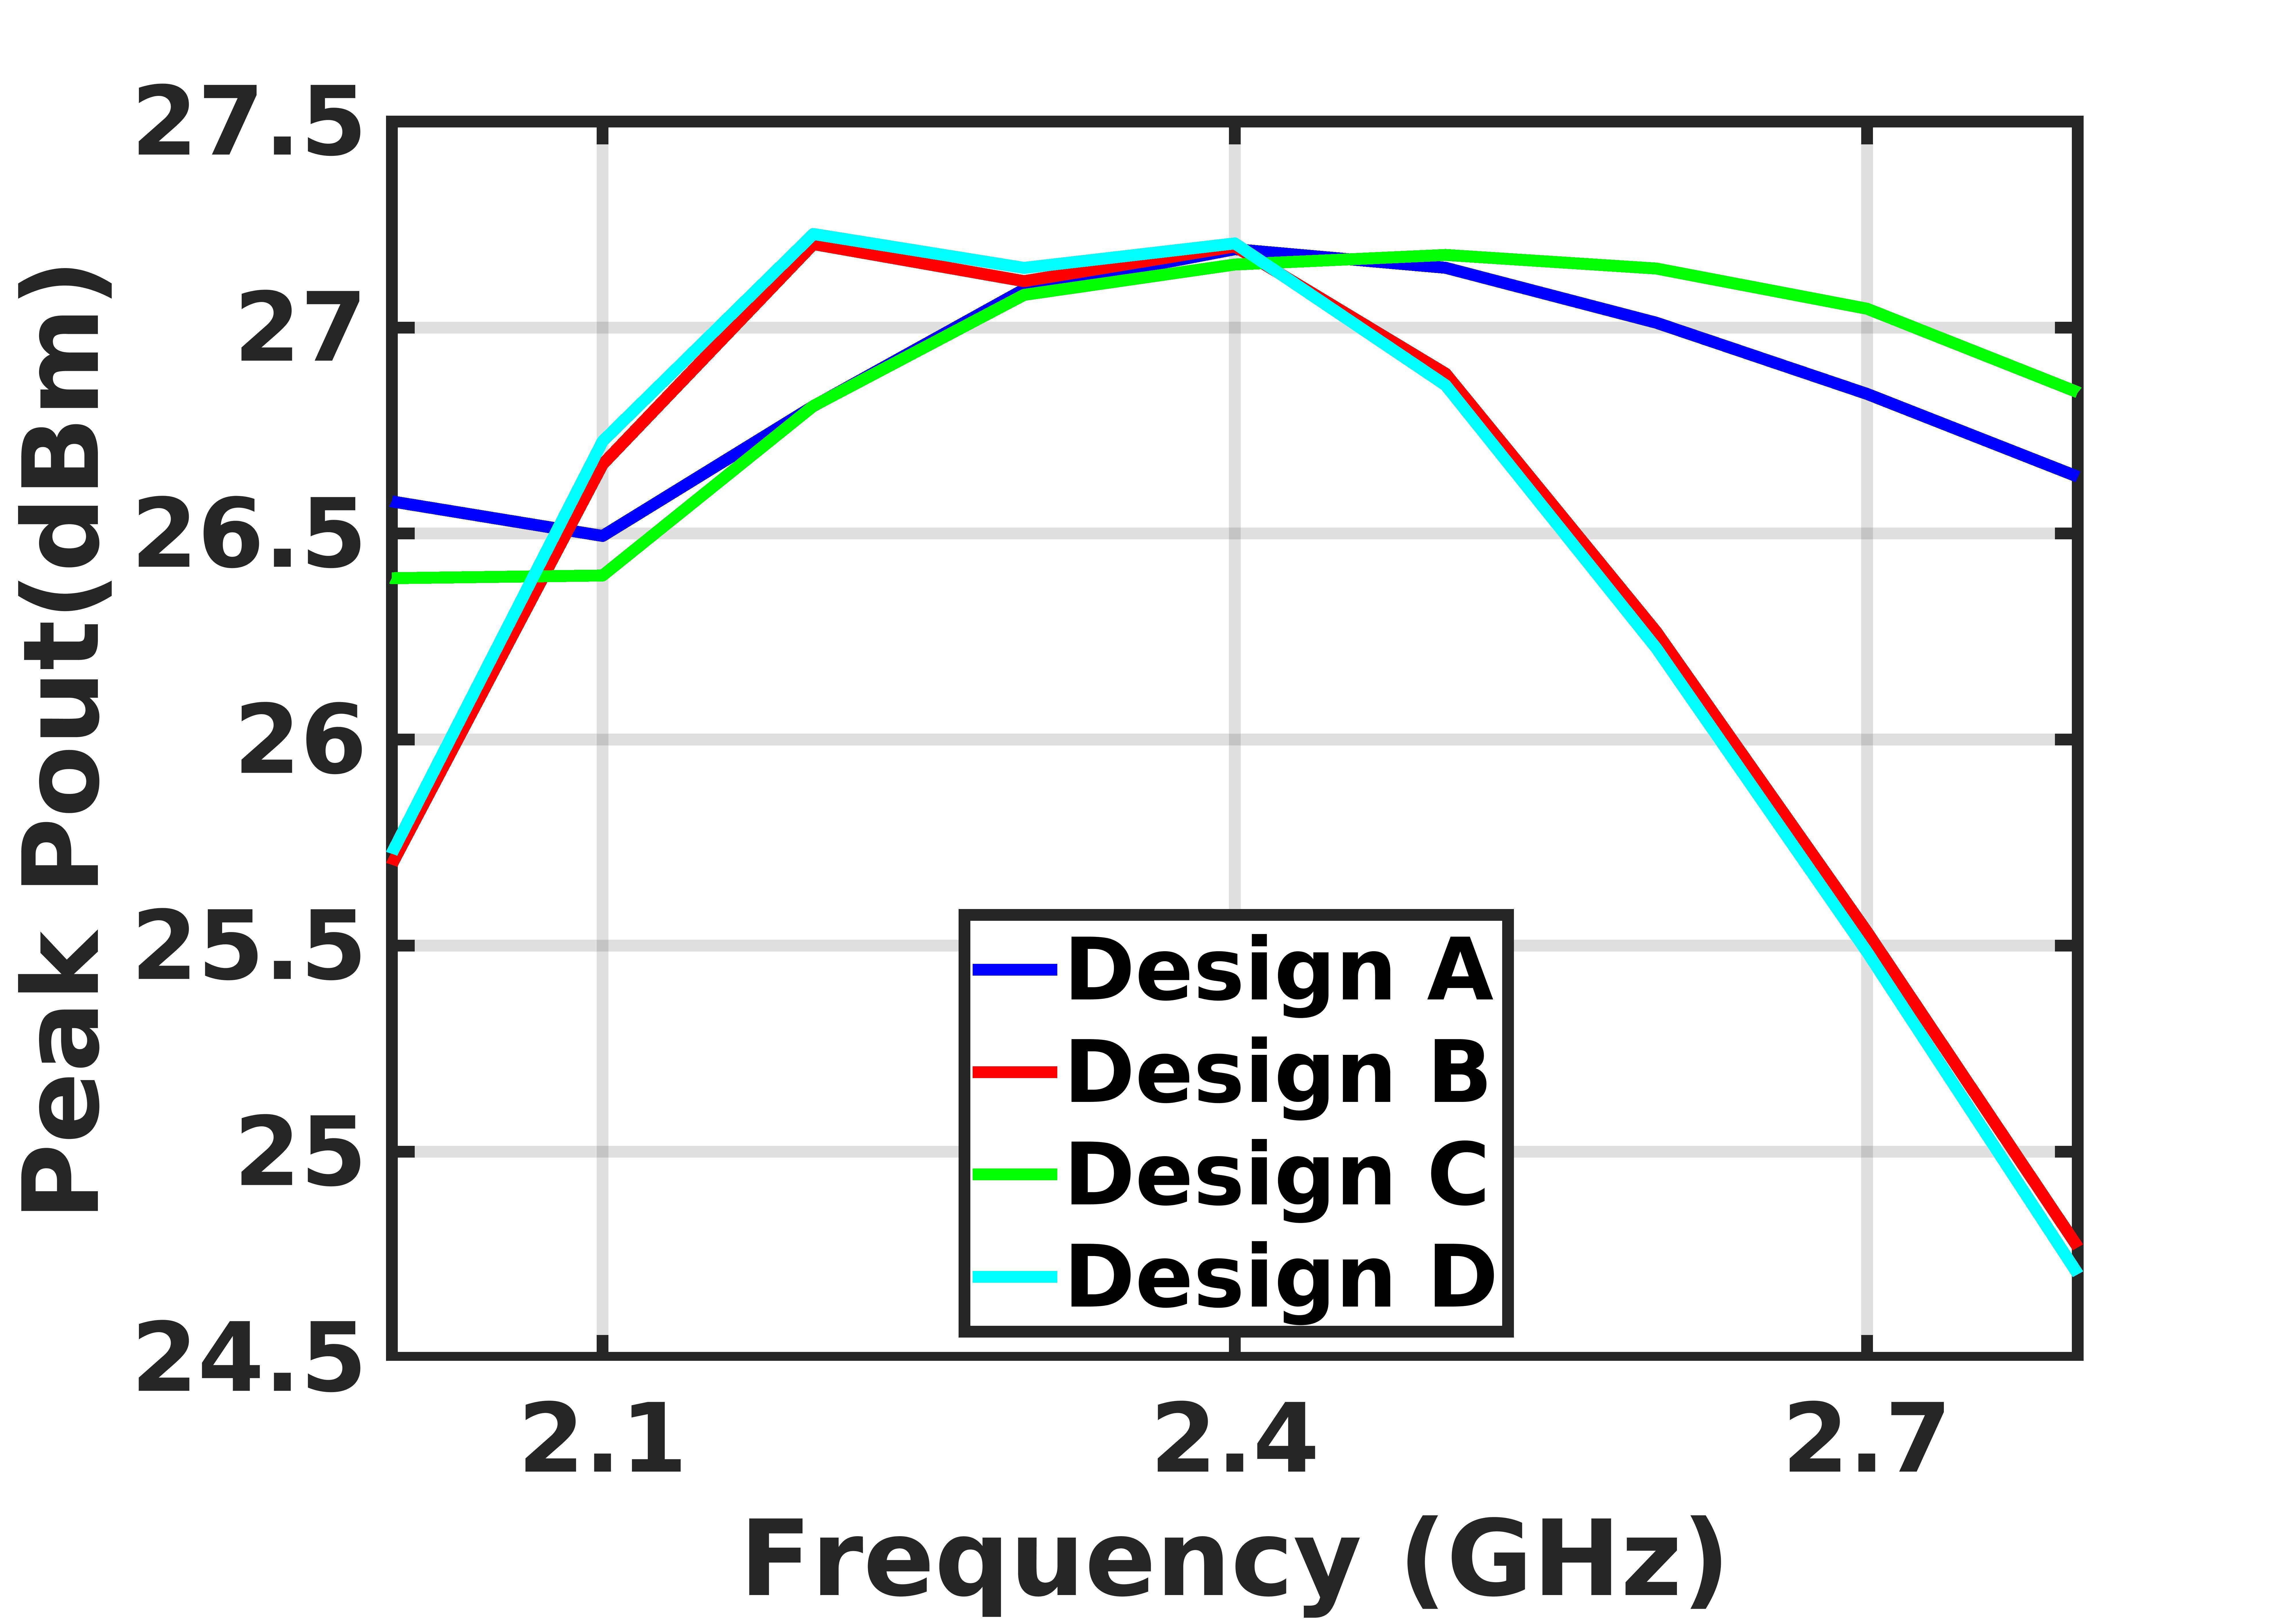
\includegraphics[width=1\textwidth]{Images/Output_Network_Comp/Comp_Pout.jpg}
\caption{}
\label{fig:Comp_Pout}
\end{subfigure}
\caption{(a) Maximum drain efficiency across frequency for 4 different output network; (b) Peak $P_{OUT}$ across frequency for 4 different output network;}
\label{fig:Comp_Pout_DE}
\vspace{-0.25in}
\end{figure}


% An example of a floating figure using the graphicx package.
% Note that \label must occur AFTER (or within) \caption.
% For figures, \caption should occur after the \includegraphics.
% Note that IEEEtran v1.7 and later has special internal code that
% is designed to preserve the operation of \label within \caption
% even when the captionsoff option is in effect. However, because
% of issues like this, it may be the safest practice to put all your
% \label just after \caption rather than within \caption{}.
%
% Reminder: the "draftcls" or "draftclsnofoot", not "draft", class
% option should be used if it is desired that the figures are to be
% displayed while in draft mode.
%
%\begin{figure}[!t]
%\centering
%\includegraphics[width=2.5in]{myfigure}
% where an .eps filename suffix will be assumed under latex, 
% and a .pdf suffix will be assumed for pdflatex; or what has been declared
% via \DeclareGraphicsExtensions.
%\caption{Simulation results for the network.}
%\label{fig_sim}
%\end{figure}

% Note that the IEEE typically puts floats only at the top, even when this
% results in a large percentage of a column being occupied by floats.


% An example of a double column floating figure using two subfigures.
% (The subfig.sty package must be loaded for this to work.)
% The subfigure \label commands are set within each subfloat command,
% and the \label for the overall figure must come after \caption.
% \hfil is used as a separator to get equal spacing.
% Watch out that the combined width of all the subfigures on a 
% line do not exceed the text width or a line break will occur.
%
%\begin{figure*}[!t]
%\centering
%\subfloat[Case I]{\includegraphics[width=2.5in]{box}%
%\label{fig_first_case}}
%\hfil
%\subfloat[Case II]{\includegraphics[width=2.5in]{box}%
%\label{fig_second_case}}
%\caption{Simulation results for the network.}
%\label{fig_sim}
%\end{figure*}
%
% Note that often IEEE papers with subfigures do not employ subfigure
% captions (using the optional argument to \subfloat[]), but instead will
% reference/describe all of them (a), (b), etc., within the main caption.
% Be aware that for subfig.sty to generate the (a), (b), etc., subfigure
% labels, the optional argument to \subfloat must be present. If a
% subcaption is not desired, just leave its contents blank,
% e.g., \subfloat[].


% An example of a floating table. Note that, for IEEE style tables, the
% \caption command should come BEFORE the table and, given that table
% captions serve much like titles, are usually capitalized except for words
% such as a, an, and, as, at, but, by, for, in, nor, of, on, or, the, to
% and up, which are usually not capitalized unless they are the first or
% last word of the caption. Table text will default to \footnotesize as
% the IEEE normally uses this smaller font for tables.
% The \label must come after \caption as always.
%
%\begin{table}[!t]
%% increase table row spacing, adjust to taste
%\renewcommand{\arraystretch}{1.3}
% if using array.sty, it might be a good idea to tweak the value of
% \extrarowheight as needed to properly center the text within the cells
%\caption{An Example of a Table}
%\label{table_example}
%\centering
%% Some packages, such as MDW tools, offer better commands for making tables
%% than the plain LaTeX2e tabular which is used here.
%\begin{tabular}{|c||c|}
%\hline
%One & Two\\
%\hline
%Three & Four\\
%\hline
%\end{tabular}
%\end{table}


% Note that the IEEE does not put floats in the very first column
% - or typically anywhere on the first page for that matter. Also,
% in-text middle ("here") positioning is typically not used, but it
% is allowed and encouraged for Computer Society conferences (but
% not Computer Society journals). Most IEEE journals/conferences use
% top floats exclusively. 
% Note that, LaTeX2e, unlike IEEE journals/conferences, places
% footnotes above bottom floats. This can be corrected via the
% \fnbelowfloat command of the stfloats package.




\section{Conclusion}
\label{section:Conclusion}
This paper presented CCF's advantage of wider bandwidth over Class F and then explained the output network's main requirement for a PA to operate in CCF mode that is if the reactive part of $1^{st}$ harmonic decreases, then the reactive part of $2^{nd}$ harmonic should increase. Further, the procedure to design the \textit{4} different output networks for the bandwidth \textit{2.1 - 2.7 GHz} were illustrated. Finally, all the \textit{4} designs were compared, and design A (with no RF choke and $L_2C_2$) was chosen because it has more constant $P_{\text{OUT}}$ in the bandwidth with the least number of components.




% conference papers do not normally have an appendix


% use section* for acknowledgment
%\section*{Acknowledgment}


%The authors would like to thank...





% trigger a \newpage just before the given reference
% number - used to balance the columns on the last page
% adjust value as needed - may need to be readjusted if
% the document is modified later
%\IEEEtriggeratref{8}
% The "triggered" command can be changed if desired:
%\IEEEtriggercmd{\enlargethispage{-5in}}

% references section

% can use a bibliography generated by BibTeX as a .bbl file
% BibTeX documentation can be easily obtained at:
% http://mirror.ctan.org/biblio/bibtex/contrib/doc/
% The IEEEtran BibTeX style support page is at:
% http://www.michaelshell.org/tex/ieeetran/bibtex/
\bibliographystyle{IEEEtran}
\bibliography{disseration.bib}
%\bibliographystyle{IEEEtran}
% argument is your BibTeX string definitions and bibliography database(s)
%\bibliography{IEEEabrv,../bib/paper}
%
% <OR> manually copy in the resultant .bbl file
% set second argument of \begin to the number of references
% (used to reserve space for the reference number labels box)
%\begin{thebibliography}{1}

%\bibitem{IEEEhowto:kopka}
%H.~Kopka and P.~W. Daly, \emph{A Guide to \LaTeX}, 3rd~ed.\hskip 1em plus
%  0.5em minus 0.4em\relax Harlow, England: Addison-Wesley, 1999.

%\end{thebibliography}



%\references{}

% that's all folks
\end{document}


